% ─────────────────────────────────────────────────────────────────────────────
%  UTILITY PATENT APPLICATION
%  Title: System and Method for Class-Conditional Synthetic Image Generation
%         via Spherical and Distributional Interpolation in a Jointly Trained
%         Adversarial Embedding Space with Adaptive Training Dynamics
%  Filing basis: 35 U.S.C. § 111(a); 37 C.F.R. § 1.52
% ─────────────────────────────────────────────────────────────────────────────

\documentclass[12pt,letterpaper]{article}

\usepackage[top=1in,bottom=1in,left=1in,right=1in]{geometry}
\usepackage{setspace}
\usepackage{amsmath,amssymb,amsthm,mathtools}
\usepackage{algorithm,algpseudocode}
\usepackage{graphicx}
\usepackage{tikz}
\usepackage{pgfplots}
\pgfplotsset{compat=1.18}
\usetikzlibrary{arrows.meta,positioning,shapes.geometric,fit,
                decorations.pathreplacing,backgrounds,calc,matrix,
                patterns,shadows,chains,scopes}
\usepackage{booktabs,multirow,array,tabularx,longtable}
\usepackage{enumitem}
\usepackage{xcolor}
\usepackage{fancyhdr}
\usepackage{titlesec}
\usepackage{caption,subcaption}
\usepackage{hyperref}
\usepackage{microtype}
\usepackage{float}
\usepackage{bm}
\usepackage{bbm}
\usepackage{parskip}
\usepackage{indentfirst}
\usepackage{tcolorbox}
\tcbuselibrary{skins,breakable}

%% Color palette
\definecolor{encoderblue}{HTML}{3B82F6}
\definecolor{slerpgreen}{HTML}{10B981}
\definecolor{decoderviolet}{HTML}{8B5CF6}
\definecolor{discrimred}{HTML}{EF4444}
\definecolor{emaorange}{HTML}{F59E0B}
\definecolor{vmfcyan}{HTML}{06B6D4}
\definecolor{phasegreen}{HTML}{22C55E}
\definecolor{phasepurple}{HTML}{A855F7}
\definecolor{sngold}{HTML}{D97706}
\definecolor{projmagenta}{HTML}{EC4899}

%% Line spacing per USPTO Rule 1.52(b)(2): 1.5 or double
\doublespacing
\setlength{\parindent}{0.5in}
\setlength{\parskip}{0pt plus 1pt}

%% Section style
\titleformat{\section}[block]
  {\normalfont\bfseries\large\centering}
  {}{0em}{\MakeUppercase}
\titleformat{\subsection}[block]
  {\normalfont\bfseries}
  {\thesubsection}{0.5em}{}
\titleformat{\subsubsection}[block]
  {\normalfont\bfseries\itshape}
  {\thesubsubsection}{0.5em}{}
\setcounter{secnumdepth}{3}

%% Convenience macros
\newcommand{\bz}{\mathbf{z}}
\newcommand{\bx}{\mathbf{x}}
\newcommand{\by}{\mathbf{y}}
\newcommand{\bw}{\mathbf{w}}
\newcommand{\bc}{\mathbf{c}}
\newcommand{\btheta}{\bm{\theta}}
\newcommand{\bphi}{\bm{\phi}}
\newcommand{\bpsi}{\bm{\psi}}
\newcommand{\bmu}{\bm{\mu}}
\newcommand{\RR}{\mathbb{R}}
\newcommand{\EE}{\mathbb{E}}
\newcommand{\NN}{\mathcal{N}}
\newcommand{\Sphere}{\mathbb{S}}

%% Claims environment
\newcounter{claimnum}
\newenvironment{claims}{%
  \setcounter{claimnum}{0}
  \begin{list}{\arabic{claimnum}.}{%
    \usecounter{claimnum}
    \setlength{\leftmargin}{2em}
    \setlength{\labelsep}{0.5em}
    \setlength{\itemsep}{0pt}
    \setlength{\parsep}{6pt plus 2pt}
  }%
}{\end{list}}

%% Header/footer
\pagestyle{fancy}
\fancyhf{}
\fancyhead[L]{\small Attorney Docket No.:\ [DOCKET]}
\fancyhead[R]{\small PATENT APPLICATION}
\fancyfoot[C]{\thepage}
\setlength{\headheight}{14pt}

\hypersetup{
  colorlinks=true,
  linkcolor=encoderblue,
  citecolor=decoderviolet,
  urlcolor=slerpgreen,
}

% ─────────────────────────────────────────────────────────────────────────────
\begin{document}
% ─────────────────────────────────────────────────────────────────────────────

% ══════════════════════════════════════════════════════════════════════════════
%  TITLE PAGE
% ══════════════════════════════════════════════════════════════════════════════
\begin{titlepage}
\centering
\vspace*{0.8in}

{\Large\bfseries UNITED STATES PATENT APPLICATION}

\vspace{0.3in}

\rule{\textwidth}{1.5pt}

\vspace{0.2in}

{\LARGE\bfseries System and Method for Class-Conditional\\[6pt]
Synthetic Image Generation via Spherical\\[6pt]
and Distributional Interpolation in a Jointly\\[6pt]
Trained Adversarial Embedding Space with\\[6pt]
Adaptive Training Dynamics}

\vspace{0.2in}

\rule{\textwidth}{1.5pt}

\vspace{0.4in}

\begin{tabular}{ll}
\textbf{Inventor:}   & [INVENTOR NAME], [CITY, STATE, COUNTRY] \\[6pt]
\textbf{Filing Type:} & Utility Patent Application \\[6pt]
\textbf{Filing Basis:} & 35 U.S.C.\ \S 111(a) \\[6pt]
\textbf{Attorney Docket:} & [DOCKET NUMBER] \\[6pt]
\textbf{Correspondence Address:} & [LAW FIRM NAME] \\
                     & [STREET ADDRESS] \\
                     & [CITY, STATE, ZIP] \\
\end{tabular}

\vspace{0.5in}

\textit{This application claims the benefit of U.S.\ Provisional Application
No.\ [PROVISIONAL NUMBER], filed [DATE], which is incorporated herein by
reference in its entirety.}

\end{titlepage}

\newpage
\tableofcontents
\newpage

% ══════════════════════════════════════════════════════════════════════════════
\section*{CROSS-REFERENCE TO RELATED APPLICATIONS}
% ══════════════════════════════════════════════════════════════════════════════

This application claims priority to U.S.\ Provisional Patent Application
No.\ [PROVISIONAL APPLICATION NUMBER], filed on [FILING DATE], entitled
``System and Method for Class-Conditional Synthetic Image Generation via
Spherical and Distributional Interpolation in a Jointly Trained Adversarial
Embedding Space with Adaptive Training Dynamics,'' the disclosure of which
is incorporated herein by reference in its entirety.

% ══════════════════════════════════════════════════════════════════════════════
\section*{STATEMENT REGARDING FEDERALLY SPONSORED RESEARCH}
% ══════════════════════════════════════════════════════════════════════════════

Not applicable.

% ══════════════════════════════════════════════════════════════════════════════
\section*{FIELD OF THE INVENTION}
% ══════════════════════════════════════════════════════════════════════════════

The present invention relates generally to the field of machine learning and
computer vision, and more particularly to systems and methods for generating
synthetic training images to address class imbalance in image datasets through
the combination of (a)~spherical linear interpolation and von~Mises--Fisher
distributional sampling in a learned hyperspherical embedding space,
(b)~class-conditional adversarial image decoding with projection
discrimination and spectral normalisation, and (c)~adaptive adversarial
training dynamics with multi-scale feature matching.

% ══════════════════════════════════════════════════════════════════════════════
\section*{BACKGROUND OF THE INVENTION}
% ══════════════════════════════════════════════════════════════════════════════

\subsection{Class Imbalance in Machine Learning}

The problem of class imbalance is one of the most pervasive and consequential
challenges encountered in applied machine learning.  Class imbalance arises
when the number of training examples belonging to different categories differs
by a substantial factor, often by one or more orders of magnitude.  In
supervised classification tasks applied to image data, this imbalance
manifests directly in model performance: classifiers trained on imbalanced
corpora exhibit systematic bias toward majority classes, achieving inflated
aggregate accuracy while producing unacceptable recall on underrepresented
categories.  This failure mode has real consequences across medical imaging,
where rare pathology classes are frequently underrepresented; in autonomous
driving, where uncommon road events must nonetheless be recognized reliably;
and in industrial quality control, where defect classes are inherently rare
relative to conforming products.

The conventional approaches to addressing class imbalance fall into two broad
families: sampling-based methods and cost-sensitive learning methods.
Cost-sensitive approaches modify the training objective to penalize
misclassification of minority examples more heavily than majority examples,
but they do not alter the fundamental information content available to the
learner and therefore provide only modest improvement when the minority class
is severely underrepresented.  Sampling-based methods, by contrast, directly
alter the composition of the training corpus, either by removing
majority-class examples through undersampling or by replicating or
synthesizing minority-class examples through oversampling.  Of these,
synthetic oversampling is generally preferred for image data because it avoids
the information loss inherent in undersampling while introducing new training
examples that can improve the generalization surface of the learned classifier.

\subsection{Limitations of Prior Interpolation-Based Oversampling}

The Synthetic Minority Over-sampling Technique (SMOTE), introduced by Chawla
and colleagues~\cite{chawla2002}, was a foundational advance in synthetic
oversampling.  In its original form, SMOTE operates directly on the raw
feature vectors of minority-class examples, selecting a minority-class
instance and one of its $k$ nearest neighbors within the same class, then
synthesizing a new example at a random position along the linear segment
connecting them in the original feature space.  Formally, for two minority
examples $\bx_i$ and $\bx_j$, SMOTE generates a synthetic example as
$\bx_{\text{syn}} = \bx_i + \lambda(\bx_j - \bx_i)$ where $\lambda$ is
drawn uniformly from $[0,1]$.

When SMOTE was originally proposed, application to raw feature vectors of
tabular or low-dimensional data was natural and well-motivated.  However, the
application of linear interpolation to image data presents a fundamental
geometric problem that has not been adequately addressed in the prior art.
The space of natural images is not a convex subset of the raw pixel space;
rather, natural images occupy a curved, low-dimensional manifold embedded in
a very high-dimensional ambient pixel space.  Linear interpolation between two
points on a curved manifold does not in general remain on the manifold; the
resulting intermediate points may correspond to blurry, physically implausible
pixel arrays that bear no resemblance to any real image.  This
manifold-departure problem is particularly severe for image data, where the
valid image manifold is highly nonlinear and where even small deviations from
the manifold produce perceptually unacceptable artifacts.

The inventor has discovered that this limitation is not merely cosmetic but
causes direct degradation in downstream classifier performance.  When
interpolated images depart from the valid image manifold, they carry
misleading statistical information about the minority class distribution, and
classifiers trained on such data learn spurious features that do not
generalize to test examples drawn from the true minority distribution.  Prior
attempts to apply SMOTE to images in the raw pixel space or in the feature
spaces of pre-trained classifiers have not adequately resolved this
fundamental geometric limitation.

\subsection{Limitations of Prior Generative Oversampling Approaches}

An alternative line of prior art employs generative models, particularly
Generative Adversarial Networks (GANs)~\cite{goodfellow2014}, to synthesize
minority-class images directly.  Under this paradigm, a GAN is trained on
available minority-class examples and then used to generate additional images
that are decoded from random latent vectors.  While this approach sidesteps
the manifold-departure problem of direct interpolation, it introduces a
distinct set of limitations.

First, generative approaches that sample from a learned prior distribution do
not provide the structured interpolation property that gives SMOTE its primary
advantage for class-balancing purposes: the ability to fill gaps in the
minority-class sample density in a principled and controlled manner.  A GAN
sampling from a broad prior distribution may repeatedly generate examples from
already-well-represented regions of the minority class manifold while failing
to generate examples that fill the specific gaps in the training corpus where
class density is lowest.

Second, GANs trained in isolation on small minority-class corpora frequently
exhibit mode collapse, generating a limited variety of outputs that fail to
capture the full diversity of the minority class distribution.  This
limitation is especially acute when the available minority-class training data
is small, which is precisely the regime in which class-balancing is most
urgently needed.

Third, prior generative oversampling methods have not established a rigorous
coupling between the interpolation operation in the latent space and the
geometric properties of that space.  When the latent space does not have a
well-defined metric structure, interpolation in that space produces results
whose relationship to the true minority-class distribution is unpredictable.
The inventor has observed that this lack of geometric grounding is a root
cause of the unreliability of prior generative oversampling approaches.

\subsection{Absence of Class Conditioning in Prior Decoder Architectures}

A further limitation of prior art approaches to synthetic image generation for
class-balancing is the failure to exploit class identity information within
the generative decoder.  In a class-imbalanced dataset, examples belonging to
different classes may occupy well-separated regions of the embedding space.
When a decoder is trained without awareness of which class its input
embeddings belong to, it must learn a single shared generative mapping that
spans multiple class-conditioned distributions.  This is particularly
problematic when the decoder architecture employs batch normalization, which
computes feature statistics over batches that may span multiple classes.

The inventor has found that decoding quality degrades substantially when the
decoder is class-unaware, particularly in the fine-grained visual details that
distinguish between similar classes.  Class-conditional information, when
properly incorporated, provides the decoder with direct guidance about which
region of the output distribution it should target, enabling more precise and
class-faithful synthetic image generation.  Prior art architectures operating
on image embedding spaces have either ignored class-conditional information
entirely or incorporated it through architectural choices that do not provide
sufficient capacity for the decoder to exploit it effectively.

\subsection{Training Instability and Parameter Trajectory Problems}

The training of adversarial image generation systems is well-known to be
unstable, and this instability is particularly pronounced when training is
conducted on the small datasets characteristic of minority-class oversampling
scenarios.  The standard GAN training objective involves a minimax game
between a generator and a discriminator, and this game does not have a
guaranteed convergence path for finite-capacity networks trained on finite
data.  The resulting training trajectories frequently exhibit mode collapse,
oscillation, and catastrophic forgetting.

One specific manifestation of this instability that has received insufficient
attention in the prior art concerns the temporal trajectory of decoder
parameters during training.  It is well established in the optimization
literature that parameter trajectories during stochastic gradient descent
exhibit substantial high-frequency oscillation, and that the time-average of
parameters along such trajectories frequently generalizes better than any
individual point on the trajectory.  This property, which underlies classical
methods such as Polyak averaging, is especially important for generative
models where individual training checkpoints may correspond to locally
degenerate solutions.  Prior art generative oversampling systems have failed
to incorporate principled parameter averaging schemes, instead using the final
training checkpoint regardless of the quality of its generative outputs
relative to other points along the training trajectory.

\subsection{Limitations of Class-Unconditional Discrimination}

Prior art discriminator architectures for GAN-based image synthesis have
predominantly employed class-unconditional critics that evaluate image
realism without regard to class identity.  The inventor has recognized that
this design choice is fundamentally mismatched with the class-conditional
generation task.  A class-unconditional discriminator can only enforce that
generated images look realistic in a class-agnostic sense, but cannot
enforce that images generated for class~$k$ actually resemble class-$k$
images specifically.  This limitation becomes acute in multi-class generation
scenarios where the decoder must produce distinct outputs for distinct
classes.

The inventor has further identified that per-layer Lipschitz stability of the
discriminator, achieved through spectral normalisation of weight
matrices~\cite{miyato2018}, provides finer-grained gradient control than
global gradient penalty alone, and that the combination of both constraints
produces more stable training dynamics than either constraint in isolation.

\subsection{Absence of Distributional Oversampling on the Hypersphere}

All prior art oversampling approaches known to the inventor operate by
pairwise interpolation between existing data points.  The inventor has
recognized that this pairwise paradigm introduces a selection bias: the
distribution of synthetic points is constrained to lie along line segments
(or geodesic arcs) connecting existing samples, and cannot cover regions of
the class distribution that are not well-served by any pair of existing
points.  A fundamentally different approach is to model the class-conditional
distribution on the embedding hypersphere directly and sample from that
distribution, generating synthetic embeddings that are not constrained to
lie between any particular pair of anchor points.

The von~Mises--Fisher (vMF) distribution~\cite{mardia2000,banerjee2005}
is the natural analog of the Gaussian distribution on the unit hypersphere.
The inventor has discovered that fitting a vMF distribution to each class's
embeddings and sampling from that distribution provides a complementary
oversampling strategy that is free from the pair-selection bias of
SLERP-based interpolation and is particularly effective when the within-class
embedding distribution is approximately unimodal on the hypersphere.

\subsection{Lack of Universal Dataset Interface}

A practical limitation that has significantly hindered the adoption of prior
art approaches to synthetic image oversampling is the absence of a universal
dataset interface.  Most prior art systems require dataset-specific
preprocessing pipelines, class-label enumeration, and image loading code that
must be rewritten for each new application.  This requirement creates
substantial engineering overhead, increases the likelihood of data-handling
bugs, and prevents straightforward comparison of results across datasets.
The inventor has recognized that the lack of a universal,
convention-based dataset interface is a significant barrier to practical
deployment of synthetic oversampling systems and has designed the present
invention to address this limitation directly through a
convention-over-configuration dataset loading strategy that requires no
dataset-specific code.

% ══════════════════════════════════════════════════════════════════════════════
\section*{SUMMARY OF THE INVENTION}
% ══════════════════════════════════════════════════════════════════════════════

The present invention provides a system and method for generating
high-quality, class-faithful synthetic images for the purpose of addressing
class imbalance in image datasets.  The invention addresses the foregoing
limitations of the prior art through a combination of novel architectural,
algorithmic, and training-dynamics innovations.

In a first aspect, the invention provides a computer-implemented method
comprising:

\begin{enumerate}[label=(\alph*),leftmargin=2em]
\item encoding images from an imbalanced training dataset to unit-norm
  embedding vectors on a high-dimensional unit hypersphere
  $\Sphere^{D-1} \subset \RR^D$ using a convolutional neural network
  augmented with an L2~normalization head;

\item synthesizing new embedding vectors by one or both of two
  complementary oversampling strategies:
  \begin{enumerate}[label=(\roman*)]
    \item \textbf{SLERP-SMOTE}: spherical linear interpolation along
      geodesic arcs connecting selected pairs of same-class embedding
      vectors, ensuring the synthesized embeddings remain precisely on the
      unit hypersphere; and
    \item \textbf{vMF-SMOTE}: fitting a von~Mises--Fisher distribution
      $\text{vMF}(\bmu_k, \kappa_k)$ to each minority class $k$ and
      sampling synthetic unit-norm embeddings directly from the fitted
      distributional model;
  \end{enumerate}

\item decoding the synthesized embedding vectors to synthetic images using
  a class-conditional convolutional decoder that concatenates a learned
  class embedding vector to the image embedding vector at the decoder
  input, incorporating non-local self-attention and spectral normalisation;

\item discriminating real from synthesized images using a projection
  discriminator~\cite{miyatokoyama2018} that computes a class-conditional
  score via inner product between a learned class embedding and the
  discriminator's penultimate representation, with spectral normalisation
  applied to all convolutional layers; and

\item training the encoder, decoder, and discriminator jointly using a
  phased schedule comprising a reconstruction-only phase followed by a
  WGAN-GP adversarial training phase with multi-scale feature matching,
  intra-class diversity repulsion loss, and adaptive adversarial loss
  weighting controlled by an EMA-smoothed Wasserstein distance monitor.
\end{enumerate}

In a second aspect, the invention provides a system comprising: a
convolutional encoder with an L2~normalization head; a dual-mode
oversampling module supporting both SLERP interpolation and vMF distributional
sampling; a class-conditional DCGAN decoder with non-local self-attention and
spectral normalisation; a projection discriminator with spectral
normalisation and multi-scale feature extraction; an adaptive adversarial
loss controller; an EMA shadow parameter manager for both encoder and decoder;
and a universal dataset interface.

In a third aspect, the invention provides a non-transitory computer-readable
medium storing instructions that, when executed, cause a processor to perform
the steps of the method described in the first aspect.

% ══════════════════════════════════════════════════════════════════════════════
\section*{BRIEF DESCRIPTION OF THE DRAWINGS}
% ══════════════════════════════════════════════════════════════════════════════

The accompanying drawings, which are incorporated herein and constitute a
part of the specification, illustrate embodiments of the invention and,
together with the description, serve to explain the principles of the
invention.

\textbf{FIG.~1} is a high-level block diagram of the complete system
architecture showing the encoder, dual-mode oversampling module (SLERP and
vMF), class-conditional decoder, projection discriminator, adaptive
$\lambda_{\text{adv}}$ controller, and EMA manager.

\textbf{FIG.~2} is a diagram illustrating the geometric relationship between
linear interpolation (LERP) and spherical linear interpolation (SLERP) on the
unit hypersphere $\Sphere^{D-1}$, showing the departure of linear
interpolation from the hypersphere surface.

\textbf{FIG.~3} is a detailed architectural diagram of the ResNet encoder
with the L2~normalization head.

\textbf{FIG.~4} is a diagram showing the SLERP oversampling procedure,
illustrating the $k$-nearest-neighbor selection and interpolation along a
class-homogeneous geodesic arc.

\textbf{FIG.~5} is a diagram illustrating the von~Mises--Fisher (vMF)
distributional sampling procedure on the unit hypersphere, showing the
class-conditional concentration parameter $\kappa$ and the mean direction
$\bmu$.

\textbf{FIG.~6} is a detailed architectural diagram of the class-conditional
DCGAN decoder showing the class embedding concatenation, transposed
convolutional layers with spectral normalisation, and non-local
self-attention block placement.

\textbf{FIG.~7} is a diagram of the non-local self-attention block used in
the decoder, showing the query, key, and value projections and the attention
weight computation.

\textbf{FIG.~8} is a detailed architectural diagram of the projection
discriminator showing the spectrally normalised strided convolutional layers,
the projection class-conditioning mechanism, and the multi-scale feature
extraction pathway.

\textbf{FIG.~9} is a timeline diagram of the phased training schedule,
showing the reconstruction-only phase and the adversarial training phase with
corresponding loss terms and the adaptive $\lambda_{\text{adv}}$ trajectory.

\textbf{FIG.~10} is a diagram of the adaptive adversarial loss weight
controller, showing the EMA-smoothed Wasserstein distance monitor and the
ramp/feedback adjustment mechanism.

\textbf{FIG.~11} is a diagram of the EMA shadow parameter manager, showing
the parameter accumulation process during training and the permanent weight
substitution at training completion for both encoder and decoder.

\textbf{FIG.~12} is a diagram of the universal dataset interface, showing
the folder-structure convention and the resulting class-labeled batch
sampling procedure.

\textbf{FIG.~13} is a flow diagram of the complete synthetic image generation
procedure following training completion.

\textbf{FIG.~14} is a diagram illustrating the cosine annealing learning rate
schedule, including the handling of schedule state during the phase transition
at epoch $0.3 \times T$.

\textbf{FIG.~15} is a diagram showing the architecture of the optional VGG-16
perceptual loss module and the feature layers used for perceptual similarity
computation.

\textbf{FIG.~16} is a diagram illustrating the intra-class diversity
repulsion loss mechanism, showing the pairwise cosine distance computation
within each class and the hinge-margin penalty.

% ══════════════════════════════════════════════════════════════════════════════
\section*{DETAILED DESCRIPTION OF THE PREFERRED EMBODIMENTS}
% ══════════════════════════════════════════════════════════════════════════════

The following detailed description is set forth to assist in understanding
the invention and is not intended to limit the scope of the invention, which
is defined by the claims appended hereto.

\subsection{System Overview}

In the preferred embodiment, the disclosed system comprises eight principal
components that cooperate to synthesize class-faithful images for addressing
class imbalance in image datasets.  These components are:

\begin{enumerate}[label=\textbf{(\arabic*)},leftmargin=2em]
  \item A convolutional encoder with an L2~normalization head
  \item A dual-mode SLERP/vMF oversampling module
  \item A class-conditional DCGAN decoder with non-local self-attention and spectral normalisation
  \item A projection discriminator with spectral normalisation
  \item An adaptive adversarial loss weight controller
  \item A multi-scale feature matching module
  \item An EMA shadow parameter manager (encoder and decoder)
  \item A universal dataset interface
\end{enumerate}

The system is trained end-to-end in a phased schedule and, upon training
completion, operates as a standalone image synthesis engine capable of
generating any requested number of synthetic images for any class in the
training dataset.

Referring to FIG.~1, the system architecture operates as follows during
training.  An input image $\bx \in \RR^{H \times W \times C}$, where $H$
and $W$ denote spatial dimensions and $C$ denotes the number of channels, is
provided to an encoder $E_{\bphi}$ parameterized by weights $\bphi$.  The
encoder maps the input image to a unit-norm embedding vector
$\bz \in \Sphere^{D-1} \subset \RR^D$, where $D$ denotes the embedding
dimensionality and $\Sphere^{D-1}$ denotes the $(D-1)$-dimensional unit
hypersphere.  The class label $y \in \{0, 1, \ldots, K-1\}$ associated with
the input image, where $K$ denotes the total number of classes, is separately
processed by a class embedding lookup
$\bm{e}_y = \mathbf{E}_c[y] \in \RR^{d_c}$, where
$\mathbf{E}_c \in \RR^{K \times d_c}$ is a learnable class embedding matrix
and $d_c$ is the class embedding dimensionality.

The unit-norm embedding $\bz$ and the class embedding $\bm{e}_y$ are
concatenated to form the conditioning vector
$\bc = [\bz; \bm{e}_y] \in \RR^{D + d_c}$, which is provided to a
class-conditional DCGAN decoder $G_{\btheta}$ parameterized by weights
$\btheta$.  The decoder reconstructs the input image as
$\hat{\bx} = G_{\btheta}(\bc)$.  A projection discriminator $D_{\bpsi}$
parameterized by weights $\bpsi$ receives either real images $\bx$ or
reconstructed images $\hat{\bx}$, together with class labels, and produces a
class-conditional real-valued critic score.  During training, the adversarial
loss, reconstruction loss, feature matching loss, and intra-class repulsion
loss are computed and used to update the parameters $\btheta$, $\bphi$, and
$\bpsi$ according to the phased training schedule described herein.  An EMA
manager maintains shadow parameters $\tilde{\btheta}$ and $\tilde{\bphi}$
that track the time-averaged encoder and decoder weights throughout training.

Upon completion of training, the dual-mode oversampling module operates on
the encoded representations of the training data.  For each minority class
$k$, the module synthesizes new embeddings either by SLERP interpolation
along geodesic arcs connecting same-class pairs, or by sampling from a fitted
vMF distribution $\text{vMF}(\bmu_k, \kappa_k)$.  These synthesized
embeddings, together with their associated class labels, are then passed
through the EMA-weight decoder $G_{\tilde{\btheta}}$ to produce synthetic
images.

\subsection{The Convolutional Encoder with L2~Normalization Head}

\subsubsection{Encoder Architecture}

In the preferred embodiment, the encoder $E_{\bphi}$ is built upon a
ResNet-18 backbone~\cite{he2016} pretrained on ImageNet.  The ResNet-18
backbone comprises four residual block groups, each group consisting of two
residual blocks with batch normalization and ReLU activations.  The four
groups operate on feature maps of spatial resolution $H/8 \times W/8$,
$H/16 \times W/16$, $H/32 \times W/32$, and $H/64 \times W/64$
respectively.  The number of feature channels in the four groups is 64, 128,
256, and 512, respectively.

Following the final residual block group, a global average pooling layer
reduces the spatial dimensions to produce a $512$-dimensional feature vector
$\mathbf{h} \in \RR^{512}$.  This feature vector is passed through an
L2~normalization head comprising a linear projection layer followed by an
L2~normalization operation.  Specifically, the linear projection is
$\mathbf{p} = \mathbf{W}_{\text{proj}}\,\mathbf{h} +
\mathbf{b}_{\text{proj}}$, where
$\mathbf{W}_{\text{proj}} \in \RR^{D \times 512}$ and
$\mathbf{b}_{\text{proj}} \in \RR^D$ are learnable parameters, and the
embedding is obtained by L2~normalization:

\begin{equation}
  \bz = \frac{\mathbf{p}}{\|\mathbf{p}\|_2},
  \label{eq:l2norm}
\end{equation}

\noindent where $\|\cdot\|_2$ denotes the Euclidean norm.  The resulting
embedding $\bz$ satisfies $\|\bz\|_2 = 1$ by construction, i.e.,
$\bz \in \Sphere^{D-1}$.  In the preferred embodiment, $D = 512$.

\subsubsection{Motivation for the L2~Normalization Head}

The L2~normalization head serves a purpose beyond merely constraining the
norm of the embedding vector.  The inventor has recognized that unit-norm
normalization induces a geometry on the embedding space that is precisely
compatible with both the spherical linear interpolation operation and the
von~Mises--Fisher distributional sampling described hereinafter.  When
embeddings are constrained to lie on $\Sphere^{D-1}$, the natural
interpolation between two embeddings is the geodesic arc connecting them on
the sphere, and the natural generative distribution is the vMF distribution.
In the absence of the L2~normalization constraint, embeddings may have
arbitrary norms, and neither SLERP nor vMF sampling produces geometrically
meaningful results.

Furthermore, the inventor has discovered that L2~normalization has a
beneficial regularizing effect on encoder training, analogous to the effect
observed in metric learning literature.  By forcing the encoder to represent
all input images as points on a fixed-radius hypersphere, the normalization
prevents the encoder from using the magnitude of the embedding vector as an
additional degree of freedom, effectively encouraging the encoder to allocate
all representational capacity to the angular structure of the embedding
space.

\subsubsection{Alternative Encoder Architectures}

It will be appreciated by those skilled in the art that the ResNet backbone
described above is not the sole architecture suitable for use as the encoder
component.  In alternative embodiments, a Vision Transformer (ViT), an
EfficientNet backbone, or a ResNet-50 backbone may be substituted.
Regardless of the choice of backbone, the L2~normalization head described in
Equation~(\ref{eq:l2norm}) is applied to the backbone output in all
embodiments of the present invention.

\subsection{Dual-Mode Oversampling: SLERP and von~Mises--Fisher}

The oversampling module of the present invention supports two complementary
strategies for synthesizing minority-class embeddings on the unit hypersphere.
The two strategies may be used individually or in combination.

\subsubsection{Strategy~I: Spherical Linear Interpolation (SLERP-SMOTE)}

\paragraph{Geometric Motivation.}

The fundamental innovation of the interpolation-based oversampling component
is the replacement of the standard linear interpolation (LERP) used in prior
art SMOTE implementations with spherical linear interpolation (SLERP).  When
embeddings lie on the unit hypersphere $\Sphere^{D-1}$, straight-line
interpolation between two points on the sphere passes through the interior
of the sphere rather than along the sphere surface, departing from the
manifold on which the real data are constrained to lie.  SLERP, by contrast,
interpolates along the geodesic arc of $\Sphere^{D-1}$ connecting the two
points, ensuring that all interpolated embeddings remain on the unit sphere.

\paragraph{The SLERP Formula.}

Let $\bz_0, \bz_1 \in \Sphere^{D-1}$ be two unit-norm vectors, and let
$\omega \in [0, \pi]$ denote the angle between them:

\begin{equation}
  \omega = \arccos\!\bigl(\bz_0 \cdot \bz_1\bigr).
  \label{eq:omega}
\end{equation}

For a given interpolation parameter $t \in [0,1]$, the SLERP interpolant is:

\begin{equation}
  \hat{\bz}(t) = \frac{\sin\bigl((1-t)\,\omega\bigr)}{\sin\omega}\,\bz_0
                + \frac{\sin\bigl(t\,\omega\bigr)}{\sin\omega}\,\bz_1.
  \label{eq:slerp}
\end{equation}

It is straightforward to verify that $\|\hat{\bz}(t)\|_2 = 1$ for all
$t \in [0,1]$, confirming that the SLERP interpolant remains on the unit
hypersphere.  Furthermore, the SLERP formula provides constant angular
velocity along the geodesic arc, meaning that equal increments in the
interpolation parameter $t$ correspond to equal angular displacements along
the arc.

\paragraph{Numerical Stability.}

When $\omega$ is close to zero ($\omega < \epsilon = 10^{-6}$), the SLERP
formula exhibits numerical instability due to division by $\sin\omega
\approx 0$.  In this degenerate case, the robust fallback is:

\begin{equation}
  \hat{\bz}(t) = \frac{(1-t)\bz_0 + t\bz_1}{\|(1-t)\bz_0 + t\bz_1\|_2}.
  \label{eq:slerp_fallback}
\end{equation}

\paragraph{Density-Weighted Interpolation Parameter.}

In one embodiment, the interpolation parameter $t$ is biased toward $0.5$ in
low-density geodesic regions and drawn uniformly in high-density regions.
Per-point $k$-NN density estimates determine the local density along each
geodesic arc, directing synthetic samples preferentially into gaps in the
minority-class distribution.

\paragraph{Cluster-Constrained $k$-NN Selection.}

In one embodiment, $k$-nearest-neighbor selection for SLERP is constrained to
within-cluster neighbors only, preventing interpolation between semantically
distant modes of the same class.  The per-class clustering uses $K$-means,
DBSCAN, hierarchical agglomerative clustering, or Gaussian mixture models,
with automatic cluster count selection.

\paragraph{$k$-Nearest Neighbor Selection and Class Homogeneity.}

For each minority-class embedding $\bz_i$, the oversampling module identifies
a set of $k = 5$ nearest neighbors within the same class using cosine
similarity.  A critical constraint is that the two anchor embeddings $\bz_0$
and $\bz_1$ are always drawn from the same class, ensuring class-faithful
interpolation.

\subsubsection{Strategy~II: von~Mises--Fisher Distributional Sampling (vMF-SMOTE)}

\paragraph{Motivation.}

The inventor has recognized that pairwise SLERP interpolation, while
geometrically principled, inherits the selection bias of all $k$-NN-based
oversampling methods: synthetic samples can only appear along geodesic arcs
connecting existing data points, leaving coverage gaps in regions of the
class distribution not well-served by any existing pair.  The
von~Mises--Fisher (vMF) distribution provides a complementary,
pair-selection-free strategy.

\paragraph{The vMF Distribution.}

The von~Mises--Fisher distribution on $\Sphere^{D-1}$ is defined by a mean
direction $\bmu \in \Sphere^{D-1}$ and a concentration parameter
$\kappa \geq 0$.  Its probability density function is:

\begin{equation}
  f_D(\bz;\, \bmu,\, \kappa) =
    C_D(\kappa)\,\exp\!\bigl(\kappa\,\bmu^\top \bz\bigr),
  \label{eq:vmf_pdf}
\end{equation}

where $C_D(\kappa) = \kappa^{D/2 - 1} /
\bigl((2\pi)^{D/2}\,I_{D/2-1}(\kappa)\bigr)$ is the normalizing constant
and $I_\nu(\cdot)$ denotes the modified Bessel function of the first kind.
When $\kappa = 0$, the vMF distribution reduces to the uniform distribution
on the sphere; as $\kappa \to \infty$, the distribution concentrates at
$\bmu$.

\paragraph{Maximum Likelihood Estimation.}

For a set of unit-norm embeddings $\{\bz_i\}_{i=1}^n$ belonging to a single
class, the MLE estimate of the mean direction is
$\hat{\bmu} = \bar{\bz} / \|\bar{\bz}\|_2$ where
$\bar{\bz} = \frac{1}{n}\sum_{i=1}^n \bz_i$.  The MLE concentration is
estimated using the Banerjee et~al.~\cite{banerjee2005} approximation:

\begin{equation}
  \hat{\kappa} \approx \frac{\bar{R}\,(D - \bar{R}^2)}{1 - \bar{R}^2},
  \label{eq:kappa_mle}
\end{equation}

where $\bar{R} = \|\bar{\bz}\|_2$ is the mean resultant length.  A
user-configurable concentration scale factor $s > 0$ is applied:
$\kappa = s \cdot \hat{\kappa}$.  Values $s > 1$ tighten the distribution
around the class mean (higher fidelity), while $s < 1$ broaden it (higher
diversity).

\paragraph{Sampling via Wood's Rejection Algorithm.}

Synthetic embeddings are sampled from $\text{vMF}(\hat{\bmu}_k, \kappa_k)$
using Wood's (1994)~\cite{wood1994} rejection algorithm, which works for any
$D \geq 2$.  The algorithm draws the axial component $W$ from a scaled Beta
distribution and combines it with a uniformly sampled tangent vector,
followed by a Householder reflection to rotate the canonical frame to the
class mean direction $\hat{\bmu}_k$.

\paragraph{Outlier Filtering.}

In one embodiment, generated vMF samples are validated against per-class
outlier detectors (Isolation Forest, One-Class SVM, or Local Outlier Factor)
fitted during the training phase.  Rejected samples are resampled up to
three times to ensure quality.

\paragraph{Synthesis Ancestry Tracking.}

In one embodiment, provenance metadata is recorded for each synthetic sample,
including parent indices (for SLERP) or the fitted $\kappa$ value (for vMF),
the synthesis method, cluster assignment, and interpolation parameter.  This
metadata supports downstream auditing and analysis.

\subsection{Class-Conditional DCGAN Decoder}

\subsubsection{Overview of Decoder Architecture}

In the preferred embodiment, the decoder $G_{\btheta}$ is based on the DCGAN
generator architecture~\cite{radford2016}, with the following modifications
introduced by the present invention: incorporation of a learned class
embedding concatenated to the image embedding at the decoder input; placement
of a non-local self-attention block at the $16 \times 16$ spatial resolution
stage; removal of batch normalization from all layers; and application of
spectral normalisation to all transposed convolutional weight matrices.

\subsubsection{Class Embedding and Input Construction}

The decoder input is constructed by concatenating the image embedding
$\bz \in \Sphere^{D-1}$ with the class embedding
$\bm{e}_y \in \RR^{d_c}$ to form the conditioning vector
$\bc = [\bz;\, \bm{e}_y] \in \RR^{D + d_c}$.  In the preferred embodiment,
$d_c = 64$.  The class embedding matrix
$\mathbf{E}_c \in \RR^{K \times 64}$ is initialized from
$\NN(0, 0.01)$ and is jointly optimized with all other parameters.

The inventor has discovered that learned class embeddings are substantially
more effective than one-hot encoding because they develop distributed
representations where semantically similar classes occupy nearby regions of
the embedding space, enabling the decoder to exploit shared structure between
related classes.

\subsubsection{Transposed Convolutional Backbone with Spectral Normalisation}

The conditioning vector $\bc$ is reshaped to a $4 \times 4$ spatial feature
map and passed through a sequence of transposed convolutional layers that
progressively double the spatial resolution.  For $128 \times 128$ output,
the decoder comprises six transposed convolutional layers at resolutions
$4 \times 4$, $8 \times 8$, $16 \times 16$, $32 \times 32$,
$64 \times 64$, and $128 \times 128$, with channel counts 512, 256, 128,
64, 64, and $C$.  Spectral normalisation is applied to each layer's weight
matrix to enforce a per-layer Lipschitz-1 constraint, stabilizing the
generator's gradient flow.

\subsubsection{Non-Local Self-Attention Block}

A non-local self-attention block~\cite{zhang2019,wang2018} is inserted at the
$16 \times 16$ spatial resolution stage.  For a feature map
$\mathbf{F} \in \RR^{16 \times 16 \times C'}$, three $1 \times 1$
projections produce query, key, and value tensors:

\begin{equation}
  \mathbf{Q} = \mathbf{W}_Q \mathbf{F}, \quad
  \mathbf{K} = \mathbf{W}_K \mathbf{F}, \quad
  \mathbf{V} = \mathbf{W}_V \mathbf{F},
  \label{eq:qkv}
\end{equation}

where $\mathbf{W}_Q, \mathbf{W}_K \in \RR^{(C'/8) \times C'}$ and
$\mathbf{W}_V \in \RR^{C' \times C'}$.  The attention map and output are:

\begin{equation}
  \mathbf{A} = \text{softmax}\!\left(\mathbf{Q}^\top \mathbf{K}\right),
  \qquad
  \mathbf{F}' = \mathbf{F} + \gamma_{\text{attn}} \cdot \mathbf{V}\mathbf{A},
  \label{eq:attn_out}
\end{equation}

where $\gamma_{\text{attn}}$ is a scalar parameter initialized to zero.
This zero initialization ensures that the self-attention block contributes
nothing at training start, allowing convolutional structure to form before
long-range attention gradually learns to augment it.

\subsection{Projection Discriminator with Spectral Normalisation}

\subsubsection{Discriminator Architecture}

In the preferred embodiment, the discriminator $D_{\bpsi}$ is a
class-conditional projection discriminator~\cite{miyatokoyama2018}
implemented as a fully convolutional network with spectrally normalised
strided convolutions.  The architecture comprises strided convolutional
layers that progressively halve the spatial resolution and double the
channel count, followed by a $4 \times 4$ final convolution producing a
scalar output.

\subsubsection{Spectral Normalisation}

Every convolutional layer in the discriminator is wrapped with spectral
normalisation~\cite{miyato2018}, which constrains the spectral norm of
each weight matrix to approximately unity via power iteration.  This
provides a per-layer Lipschitz-1 constraint that complements the global
gradient penalty, producing finer-grained gradient stability.  Formally,
for a weight matrix $\mathbf{W}$, the spectrally normalised weight is:

\begin{equation}
  \bar{\mathbf{W}} = \frac{\mathbf{W}}{\sigma(\mathbf{W})},
  \label{eq:sn}
\end{equation}

where $\sigma(\mathbf{W})$ denotes the largest singular value of
$\mathbf{W}$, estimated via one step of power iteration per training step.

\subsubsection{Projection Class Conditioning}

The projection discriminator computes a class-conditional critic score as:

\begin{equation}
  D_{\bpsi}(\bx, y) = \bw^\top \phi(\bx) +
    \mathbf{V}[y]^\top \cdot
    \text{GAP}\!\bigl(\phi(\bx)\bigr),
  \label{eq:proj_disc}
\end{equation}

where $\phi(\bx)$ denotes the penultimate feature representation,
$\bw$ is the final linear weight, $\text{GAP}(\cdot)$ denotes global
average pooling, and $\mathbf{V} \in \RR^{K \times C_{\text{pen}}}$ is a
learned class embedding table in the discriminator.  The inner product
$\mathbf{V}[y]^\top \cdot \text{GAP}(\phi(\bx))$ provides a
class-conditional bias that enables the discriminator to evaluate whether
a generated image is realistic \emph{for its target class}, not merely
realistic in a class-agnostic sense.

\subsubsection{Multi-Scale Feature Extraction}

The discriminator provides intermediate feature maps extracted at three
evenly-spaced depths (early, middle, and late convolutional stages) for
multi-scale feature matching.  The feature matching loss weights are
$[0.1, 0.3, 0.6]$, progressively emphasizing semantic features over
low-level texture features.

\subsubsection{Gradient Penalty}

The WGAN-GP gradient penalty~\cite{gulrajani2017} is applied:

\begin{equation}
  \mathcal{L}_{\text{GP}} = \lambda_{\text{GP}}\,
    \EE_{\hat{\bx}}\!\left[
      \bigl(\|\nabla_{\hat{\bx}} D_{\bpsi}(\hat{\bx}, y)\|_2 - 1\bigr)^2
    \right],
  \label{eq:gp}
\end{equation}

where $\hat{\bx} = \epsilon\,\bx_{\text{real}} +
(1 - \epsilon)\,\bx_{\text{fake}}$ with $\epsilon \sim \text{Uniform}[0,1]$,
and $\lambda_{\text{GP}} = 10$.  The combination of spectral normalisation
(per-layer) and gradient penalty (global) provides a hybrid Lipschitz
constraint that is empirically more stable than either alone.

\subsubsection{No Batch Normalization}

Consistent with the spectral normalisation framework, the discriminator uses
no batch normalization.  Batch normalization in the discriminator is
incompatible with the gradient penalty because it makes per-sample gradients
depend on all other batch samples.

\subsection{Phased Training with Adaptive Adversarial Dynamics}

\subsubsection{Phased Training Schedule}

The present invention divides the total training duration of $T$ epochs into
two phases.  In Phase~1, occupying epochs $0$ through $\lfloor 0.3\,T
\rfloor$, training is conducted exclusively with the reconstruction loss.
In Phase~2, occupying epochs $\lfloor 0.3\,T \rfloor$ through $T$, the full
adversarial objective is activated.

\subsubsection{Reconstruction Loss}

\begin{equation}
  \mathcal{L}_{\text{recon}} =
    \underbrace{\|\bx - \hat{\bx}\|_2^2}_{\text{MSE}} +
    0.5\,\underbrace{\|\bx - \hat{\bx}\|_1}_{\text{L1}} +
    0.05\,\underbrace{\sum_{\ell \in \mathcal{L}_{\text{vgg}}}
      \|\phi_\ell(\bx) - \phi_\ell(\hat{\bx})\|_1}_{\text{Perceptual}},
  \label{eq:recon}
\end{equation}

where $\phi_\ell(\cdot)$ denotes VGG-16 features from layers
\texttt{relu1\_2}, \texttt{relu2\_2}, \texttt{relu3\_3}, and
\texttt{relu4\_3}.

\subsubsection{Adversarial and Feature Matching Losses}

The discriminator loss is:

\begin{equation}
  \mathcal{L}_D = -\EE\!\bigl[D_{\bpsi}(\bx, y)\bigr]
    + \EE\!\bigl[D_{\bpsi}(\hat{\bx}, y)\bigr]
    + \mathcal{L}_{\text{GP}}.
  \label{eq:disc}
\end{equation}

The multi-scale feature matching loss is:

\begin{equation}
  \mathcal{L}_{\text{FM}} = \sum_{i=1}^{3}
    w_i \cdot \bigl\|\mathbf{f}_i(\bx) - \mathbf{f}_i(\hat{\bx})\bigr\|_1,
  \quad
  (w_1, w_2, w_3) = (0.1, 0.3, 0.6),
  \label{eq:fm}
\end{equation}

where $\mathbf{f}_i(\cdot)$ denotes feature maps at discriminator depth $i$
(texture, structure, and semantic levels, respectively).

\subsubsection{Intra-Class Diversity Repulsion Loss}

To prevent per-class mode collapse, the invention introduces an intra-class
diversity repulsion loss that penalizes excessive cosine similarity between
embeddings of the same class within each minibatch:

\begin{equation}
  \mathcal{L}_{\text{repulse}} = \frac{1}{K} \sum_{k=1}^{K}
    \frac{1}{|\mathcal{P}_k|} \sum_{(i,j) \in \mathcal{P}_k}
    \max\!\bigl(0,\; \bz_i^\top \bz_j - m\bigr),
  \label{eq:repulse}
\end{equation}

where $\mathcal{P}_k$ is the set of distinct embedding pairs within class
$k$ in the current minibatch and $m$ is the cosine margin threshold.  This
loss encourages the encoder to spread embeddings across the hyperspherical
cap assigned to each class, improving the diversity of subsequent SLERP
interpolation and vMF sampling.

\subsubsection{Adaptive Adversarial Loss Weight}

A key innovation of the present invention is the adaptive adversarial loss
weight $\lambda_{\text{adv}}$ that automatically adjusts the contribution
of the adversarial loss to the generator objective based on training
progress.  The adaptive controller operates as follows:

\begin{enumerate}[label=\textbf{(\arabic*)},leftmargin=2em]
  \item The Wasserstein distance estimate
    $\hat{W} = D_{\bpsi}(\bx, y) - D_{\bpsi}(\hat{\bx}, y)$ is computed
    at each discriminator step.

  \item An EMA-smoothed Wasserstein distance is maintained:
    $\bar{W}_t = 0.99\,\bar{W}_{t-1} + 0.01\,\hat{W}_t$.

  \item At the end of each epoch, the change
    $\Delta W = \bar{W}_{\text{current}} - \bar{W}_{\text{current}-10}$ is
    computed over a sliding window of 10 epochs.

  \item If $\Delta W < -0.01$ (Wasserstein distance decreasing, GAN
    improving), then $\lambda_{\text{adv}} \leftarrow
    \min(\lambda_{\text{adv}} + 0.005,\; 0.50)$.

  \item If $\Delta W > 0.01$ (Wasserstein distance increasing, GAN
    struggling), then $\lambda_{\text{adv}} \leftarrow
    \max(\lambda_{\text{adv}} - 0.005,\; 0.01)$.

  \item During the initial warmup period (before 10 epochs of adversarial
    history are available), $\lambda_{\text{adv}}$ follows a linear ramp
    from $0.05$ to $0.20$ over the adversarial phase.
\end{enumerate}

This feedback mechanism prevents the adversarial loss from overwhelming the
reconstruction loss when the GAN is struggling (which would cause training
instability) and allows the adversarial loss to contribute more strongly
when the GAN is converging well (which produces sharper images).

\subsubsection{Combined Generator Objective}

The complete generator training objective in Phase~2 is:

\begin{equation}
  \mathcal{L}_{\text{total}} =
    \mathcal{L}_{\text{recon}}
    + \lambda_{\text{adv}}\,\mathcal{L}_G
    + 0.1\,\mathcal{L}_{\text{FM}}
    + \lambda_{\text{repulse}}\,\mathcal{L}_{\text{repulse}},
  \label{eq:total}
\end{equation}

where $\lambda_{\text{adv}}$ is adaptively controlled as described above
and $\mathcal{L}_G = -\EE[D_{\bpsi}(\hat{\bx}, y)]$ is the WGAN generator
loss.

\subsubsection{Optimizer Configuration}

Both the encoder-decoder system and the discriminator are optimized with
Adam~\cite{kingma2015} with $\beta_1 = 0.5$ and $\beta_2 = 0.999$, and
learning rate $\eta = 0.0002$.  A cosine annealing schedule reduces the
learning rate to $\eta_{\min} = 10^{-5}$ over the full training duration:

\begin{equation}
  \eta_t = \eta_{\min} + \frac{1}{2}(\eta_0 - \eta_{\min})
    \left(1 + \cos\!\left(\frac{t}{T}\,\pi\right)\right).
  \label{eq:lr}
\end{equation}

The discriminator is updated $n_{\text{disc}} = 5$ times per generator step.
Gradient norms are clipped to a maximum of $1.0$ for the generator.

\subsection{Exponential Moving Average of Encoder and Decoder Parameters}

\subsubsection{Dual EMA Accumulation}

The EMA shadow parameter manager maintains parallel parameter sets
$\tilde{\btheta}$ and $\tilde{\bphi}$ for both the decoder and the encoder,
respectively.  After each gradient update step, both sets are updated:

\begin{equation}
  \tilde{\btheta}_t = \mu\,\tilde{\btheta}_{t-1} + (1 - \mu)\,\btheta_t,
  \qquad
  \tilde{\bphi}_t = \mu\,\tilde{\bphi}_{t-1} + (1 - \mu)\,\bphi_t,
  \label{eq:ema}
\end{equation}

where $\mu = 0.9999$.  EMA accumulation is active throughout \emph{all}
training phases (both Phase~1 and Phase~2), as the inventor has found that
EMA-smoothing of the encoder improves the quality of the embedding space for
downstream SLERP and vMF synthesis.

\subsubsection{Post-Training Weight Substitution}

At training completion, the EMA shadow parameters are permanently substituted
for the main parameters in both encoder and decoder, and the resulting models
are saved as the production models.  EMA shadow parameters are maintained at
FP32 precision regardless of the training precision to avoid rounding-error
accumulation.

\subsection{Universal Dataset Interface}

The universal dataset interface accepts any image dataset organized
according to the \texttt{ImageFolder} convention (one subdirectory per class,
with the subdirectory name serving as the class label).  Automatic class
discovery, label encoding, and image preprocessing (resize, normalize to
ImageNet statistics) are performed without any dataset-specific code.  The
target resolution is $128 \times 128$ in the preferred embodiment.

\subsection{Checkpoint Protocol}

The training pipeline saves complete checkpoints at each epoch, including
encoder, decoder, and discriminator parameters; EMA shadow parameters for
both encoder and decoder; all optimizer and scheduler states; the current
epoch index, phase index, and adaptive $\lambda_{\text{adv}}$ state.
Training can be seamlessly resumed from any checkpoint.

% ══════════════════════════════════════════════════════════════════════════════
%  ILLUSTRATIVE TABLES
% ══════════════════════════════════════════════════════════════════════════════

\subsection{Hyperparameters of the Preferred Embodiment}

\begin{table}[H]
\centering
\caption{Principal Hyperparameters}
\label{tab:hyper}
\small
\begin{tabular}{@{}llll@{}}
\toprule
\textbf{Component} & \textbf{Parameter} & \textbf{Symbol} & \textbf{Value} \\
\midrule
\multirow{2}{*}{Encoder}
  & Embedding dim     & $D$                       & 512 \\
  & Backbone          & —                         & ResNet-18 \\
\midrule
\multirow{3}{*}{SLERP}
  & $k$-neighbors     & $k$                       & 5 \\
  & Fallback $\epsilon$ & $\epsilon$              & $10^{-6}$ \\
  & Density-weighted $t$ & —                      & Optional \\
\midrule
\multirow{2}{*}{vMF}
  & Concentration scale & $s$                     & $1.0$ (default) \\
  & Sampling algorithm  & —                       & Wood (1994) \\
\midrule
\multirow{2}{*}{Decoder}
  & Class embedding dim & $d_c$                   & 64 \\
  & Attn $\gamma$ init  & $\gamma_{\text{attn}}$  & $0.0$ \\
\midrule
\multirow{2}{*}{Discriminator}
  & Normalisation       & —                       & SN + GP hybrid \\
  & FM weights          & $(w_1,w_2,w_3)$         & $(0.1,0.3,0.6)$ \\
\midrule
\multirow{6}{*}{Training}
  & Learning rate       & $\eta$                  & $2 \times 10^{-4}$ \\
  & Adam $\beta_1,\beta_2$ & —                   & $0.5,\; 0.999$ \\
  & GP coefficient      & $\lambda_{\text{GP}}$   & 10.0 \\
  & EMA decay           & $\mu$                   & 0.9999 \\
  & Phase boundary      & —                       & 30\% of epochs \\
  & Disc steps / gen step & $n_{\text{disc}}$     & 5 \\
\midrule
\multirow{3}{*}{Adaptive $\lambda_{\text{adv}}$}
  & Initial value       & —                       & 0.05 \\
  & Range               & —                       & $[0.01,\; 0.50]$ \\
  & EMA smoothing       & —                       & 0.99 \\
\bottomrule
\end{tabular}
\end{table}

\begin{table}[H]
\centering
\caption{Decoder Architecture for $128 \times 128$ Output Resolution}
\label{tab:arch}
\small
\begin{tabular}{@{}lllll@{}}
\toprule
\textbf{Layer} & \textbf{Type} & \textbf{Output Size} & \textbf{Norm} & \textbf{Note} \\
\midrule
Input        & Linear + Reshape & $4 \times 4 \times 512$   & SN & — \\
Block 1      & ConvT $4\times4$ s2p1 & $8 \times 8 \times 256$  & SN & — \\
Block 2      & ConvT $4\times4$ s2p1 & $16 \times 16 \times 128$ & SN & — \\
Self-Attn    & Non-local SA    & $16 \times 16 \times 128$ & — & $\gamma=0$ init \\
Block 3      & ConvT $4\times4$ s2p1 & $32 \times 32 \times 64$  & SN & — \\
Block 4      & ConvT $4\times4$ s2p1 & $64 \times 64 \times 64$  & SN & — \\
Output       & ConvT $4\times4$ s2p1 & $128 \times 128 \times C$ & — & Tanh \\
\bottomrule
\end{tabular}
\end{table}

\begin{table}[H]
\centering
\caption{Projection Discriminator Architecture for $128 \times 128$ Input}
\label{tab:disc_arch}
\small
\begin{tabular}{@{}lllll@{}}
\toprule
\textbf{Layer} & \textbf{Type} & \textbf{Output Size} & \textbf{Norm} & \textbf{Feature Extract} \\
\midrule
Conv 1       & Conv $4\times4$ s2p1 & $64 \times 64 \times 64$  & SN & \checkmark\ (texture) \\
Conv 2       & Conv $4\times4$ s2p1 & $32 \times 32 \times 128$ & SN & — \\
Conv 3       & Conv $4\times4$ s2p1 & $16 \times 16 \times 256$ & SN & \checkmark\ (structure) \\
Conv 4       & Conv $4\times4$ s2p1 & $8 \times 8 \times 512$   & SN & — \\
Conv 5       & Conv $4\times4$ s2p1 & $4 \times 4 \times 512$   & SN & \checkmark\ (semantic) \\
Final        & Conv $4\times4$ s1p0 & $1 \times 1 \times 1$     & SN & — \\
\midrule
Projection   & $\mathbf{V}[y]^\top \cdot \text{GAP}(\cdot)$ & scalar & — & Class-cond.\ bias \\
\bottomrule
\end{tabular}
\end{table}

% ══════════════════════════════════════════════════════════════════════════════
%  ILLUSTRATIVE FIGURES
% ══════════════════════════════════════════════════════════════════════════════

\subsection{Illustrative Figures}

%% ─── FIG 1: System Architecture ─────────────────────────────────────────────
\begin{figure}[H]
\centering
\resizebox{\textwidth}{!}{%
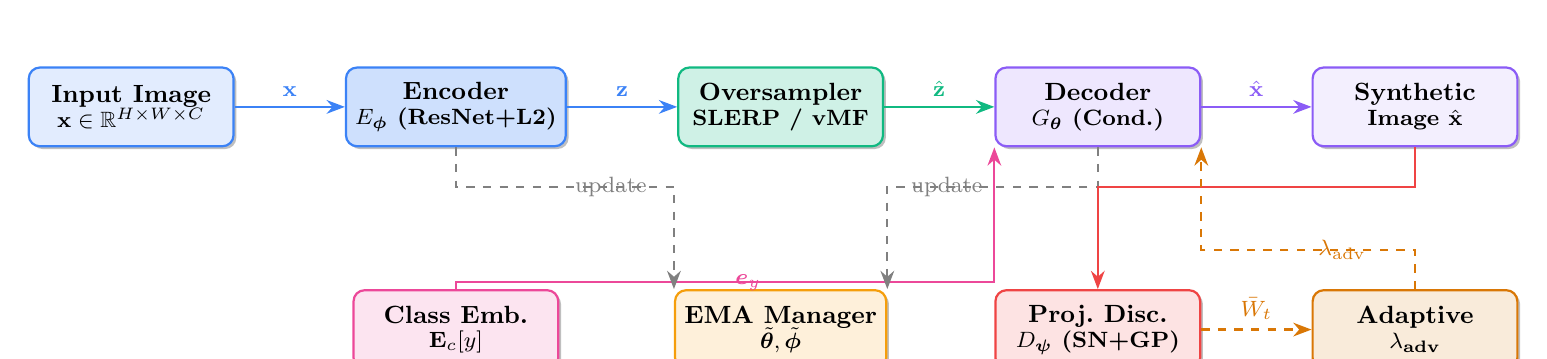
\begin{tikzpicture}[
  box/.style={draw, rectangle, rounded corners=4pt,
              minimum width=2.6cm, minimum height=1cm,
              font=\small\bfseries, align=center, thick,
              drop shadow={shadow xshift=1pt, shadow yshift=-1pt}},
  arr/.style={-Stealth, thick},
  dasharr/.style={-Stealth, thick, dashed, gray},
  node distance=0.8cm and 1.4cm
]

%% Row 1: Main forward path
\node[box, fill=encoderblue!15, draw=encoderblue]
  (img) {Input Image\\[-2pt]{\footnotesize $\bx \in \RR^{H\times W\times C}$}};

\node[box, fill=encoderblue!25, draw=encoderblue, right=1.4cm of img]
  (enc) {Encoder\\[-2pt]{\footnotesize $E_{\bphi}$ (ResNet+L2)}};

\node[box, fill=slerpgreen!20, draw=slerpgreen, right=1.4cm of enc]
  (over) {Oversampler\\[-2pt]{\footnotesize SLERP / vMF}};

\node[box, fill=decoderviolet!15, draw=decoderviolet, right=1.4cm of over]
  (dec) {Decoder\\[-2pt]{\footnotesize $G_{\btheta}$ (Cond.)}};

\node[box, fill=decoderviolet!10, draw=decoderviolet, right=1.4cm of dec]
  (out) {Synthetic\\[-2pt]{\footnotesize Image $\hat{\bx}$}};

%% Row 2: Conditioning and auxiliary — aligned horizontally
\node[box, fill=projmagenta!15, draw=projmagenta, below=1.8cm of enc]
  (cls) {Class Emb.\\[-2pt]{\footnotesize $\mathbf{E}_c[y]$}};

\node[box, fill=emaorange!15, draw=emaorange, below=1.8cm of over]
  (ema) {EMA Manager\\[-2pt]{\footnotesize $\tilde{\btheta}, \tilde{\bphi}$}};

\node[box, fill=discrimred!15, draw=discrimred, below=1.8cm of dec]
  (disc) {Proj.\ Disc.\\[-2pt]{\footnotesize $D_{\bpsi}$ (SN+GP)}};

\node[box, fill=sngold!15, draw=sngold, below=1.8cm of out]
  (adapt) {Adaptive\\[-2pt]{\footnotesize $\lambda_{\text{adv}}$}};

%% Main forward path arrows
\draw[arr, encoderblue] (img) -- (enc) node[midway,above]{\footnotesize $\bx$};
\draw[arr, encoderblue] (enc) -- (over) node[midway,above]{\footnotesize $\bz$};
\draw[arr, slerpgreen]  (over) -- (dec) node[midway,above]{\footnotesize $\hat{\bz}$};
\draw[arr, decoderviolet](dec) -- (out) node[midway,above]{\footnotesize $\hat{\bx}$};

%% Class embedding to decoder
\draw[arr, projmagenta] (cls) -- ++(0,0.6) -| (dec.south west)
  node[near start, right, font=\footnotesize]{$\bm{e}_y$};

%% EMA update (dashed)
\draw[dasharr] (enc.south) -- ++(0,-0.5) -| (ema.north west)
  node[near start, right, font=\footnotesize]{update};
\draw[dasharr] (dec.south) -- ++(0,-0.5) -| (ema.north east)
  node[near start, left, font=\footnotesize]{update};

%% Discriminator connections
\draw[arr, discrimred] (out.south) -- ++(0,-0.5) -| (disc.north)
  node[near start, right, font=\footnotesize]{};
\draw[dasharr, sngold] (disc) -- (adapt)
  node[midway,above,font=\footnotesize]{$\bar{W}_t$};
\draw[dasharr, sngold] (adapt.north) -- ++(0,0.5) -| (dec.south east)
  node[near start, right, font=\footnotesize]{$\lambda_{\text{adv}}$};

\end{tikzpicture}%
}% end resizebox
\caption{Complete system architecture.  The encoder maps input images to
unit-norm embeddings on $\Sphere^{D-1}$.  The dual-mode oversampler
synthesizes new embeddings via SLERP or vMF sampling.  The class-conditional
decoder generates synthetic images.  The projection discriminator with
spectral normalisation provides class-conditional adversarial feedback.  The
adaptive $\lambda_{\text{adv}}$ controller adjusts adversarial contribution
based on EMA-smoothed Wasserstein distance.  The EMA manager tracks both
encoder and decoder parameters.}
\label{fig:system}
\end{figure}

%% ─── FIG 2: LERP vs SLERP ──────────────────────────────────────────────────
\begin{figure}[H]
\centering
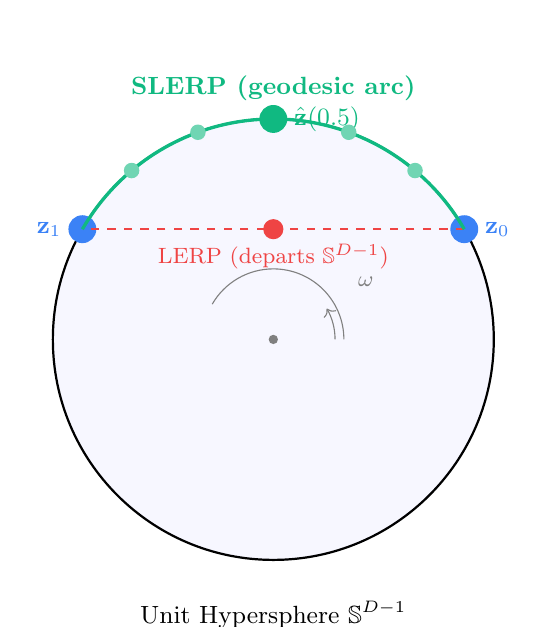
\begin{tikzpicture}[scale=2.8]
  %% Draw unit circle with subtle fill
  \draw[thick, fill=blue!3] (0,0) circle (1cm);

  %% Two anchor points (symmetric about vertical axis)
  \coordinate (z0) at ({cos(30)},{sin(30)});
  \coordinate (z1) at ({cos(150)},{sin(150)});
  \fill[encoderblue] (z0) circle (1.8pt)
    node[right=4pt, font=\small\bfseries]{$\bz_0$};
  \fill[encoderblue] (z1) circle (1.8pt)
    node[left=4pt, font=\small\bfseries]{$\bz_1$};

  %% LERP chord (departs sphere)
  \draw[thick, discrimred, dashed] (z0) -- (z1);
  \coordinate (lerpmid) at ({(cos(30)+cos(150))/2},{(sin(30)+sin(150))/2});
  \fill[discrimred] (lerpmid) circle (1.3pt);
  \node[discrimred, font=\footnotesize, below=2pt of lerpmid]
    {LERP (departs $\Sphere^{D-1}$)};

  %% SLERP arc (along the sphere surface)
  \draw[very thick, slerpgreen, domain=30:150, samples=80]
    plot ({cos(\x)},{sin(\x)});
  \node[slerpgreen, font=\small\bfseries] at (0,1.14)
    {SLERP (geodesic arc)};

  %% Midpoint on arc
  \fill[slerpgreen] ({cos(90)},{sin(90)}) circle (1.8pt)
    node[right=4pt, slerpgreen, font=\small\bfseries]{$\hat{\bz}(0.5)$};

  %% Intermediate SLERP points (constant angular velocity)
  \foreach \a in {50,70,110,130} {
    \fill[slerpgreen!60] ({cos(\a)},{sin(\a)}) circle (1pt);
  }

  %% Angle arc
  \draw[thin,->, gray] (0.28,0) arc (0:30:0.28);
  \draw[thin, gray] (0.32,0) arc (0:150:0.32);
  \node[gray, font=\footnotesize] at (0.42,0.26) {$\omega$};

  %% Origin dot
  \fill[gray] (0,0) circle (0.6pt);

  %% Label below circle
  \node[font=\small] at (0,-1.25) {Unit Hypersphere $\Sphere^{D-1}$};
\end{tikzpicture}
\caption{Geometric comparison of LERP vs.\ SLERP on the unit hypersphere.
LERP traverses the chord interior and departs from $\Sphere^{D-1}$, while
SLERP traces the geodesic arc and remains on the manifold.  Intermediate
points (light green) show constant angular velocity.}
\label{fig:slerp_geom}
\end{figure}

%% ─── FIG 3: Phased Training ────────────────────────────────────────────────
\begin{figure}[H]
\centering
\resizebox{0.95\textwidth}{!}{%
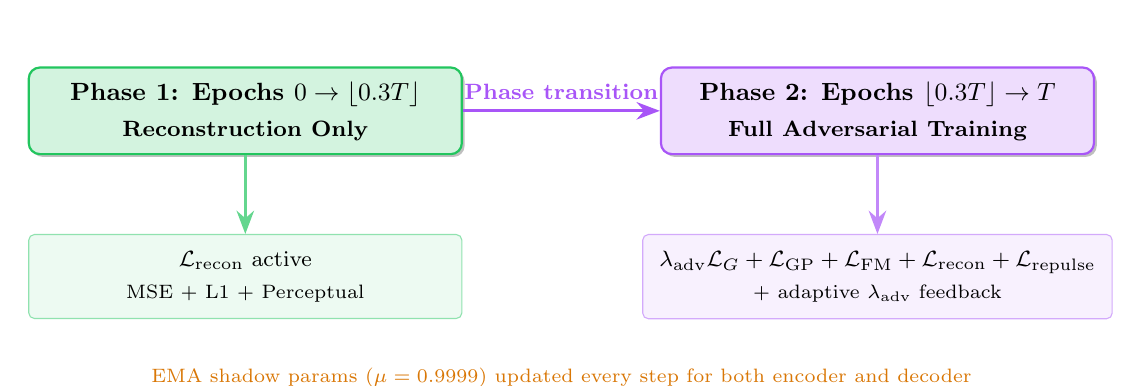
\begin{tikzpicture}[
  phase/.style={draw, rectangle, rounded corners=4pt,
                minimum width=5.5cm, minimum height=1.1cm,
                font=\small\bfseries, align=center, thick,
                drop shadow={shadow xshift=1pt, shadow yshift=-1pt}},
  lossbox/.style={draw, rectangle, rounded corners=2pt,
                  minimum width=5.5cm, font=\footnotesize, align=center,
                  inner sep=6pt},
  arr/.style={-Stealth, very thick},
]
  %% Phase boxes — horizontally centered
  \node[phase, fill=phasegreen!20, draw=phasegreen] (p1)
    {Phase 1: Epochs $0 \to \lfloor 0.3T \rfloor$\\[2pt]
     \footnotesize Reconstruction Only};

  \node[phase, fill=phasepurple!20, draw=phasepurple, right=2.5cm of p1] (p2)
    {Phase 2: Epochs $\lfloor 0.3T \rfloor \to T$\\[2pt]
     \footnotesize Full Adversarial Training};

  %% Loss term boxes (aligned below phase boxes)
  \node[lossbox, fill=phasegreen!8, draw=phasegreen!50, below=1cm of p1] (l1)
    {$\mathcal{L}_{\text{recon}}$ active\\[2pt]
     {\scriptsize MSE + L1 + Perceptual}};

  \node[lossbox, fill=phasepurple!8, draw=phasepurple!50, below=1cm of p2] (l2)
    {$\lambda_{\text{adv}}\mathcal{L}_G +
     \mathcal{L}_{\text{GP}} +
     \mathcal{L}_{\text{FM}} +
     \mathcal{L}_{\text{recon}} +
     \mathcal{L}_{\text{repulse}}$\\[2pt]
     {\scriptsize + adaptive $\lambda_{\text{adv}}$ feedback}};

  %% Transition arrow
  \draw[arr, phasepurple] (p1) -- (p2)
    node[midway, above, font=\footnotesize\bfseries]{Phase transition};

  %% Vertical connection arrows
  \draw[arr, phasegreen!70] (p1.south) -- (l1.north);
  \draw[arr, phasepurple!70] (p2.south) -- (l2.north);

  %% EMA annotation centered below both
  \node[font=\scriptsize, sngold,
        below=0.5cm of $(l1.south)!0.5!(l2.south)$]
    {EMA shadow params ($\mu=0.9999$) updated every step for both encoder and decoder};
\end{tikzpicture}%
}% end resizebox
\caption{Phased training schedule with adaptive adversarial dynamics.
Phase~1 establishes reconstruction fidelity.  Phase~2 activates WGAN-GP
adversarial training with projection discrimination, multi-scale feature
matching, intra-class repulsion, and adaptive $\lambda_{\text{adv}}$.}
\label{fig:phases}
\end{figure}

%% ─── FIG 4: vMF Sampling ───────────────────────────────────────────────────
\begin{figure}[H]
\centering
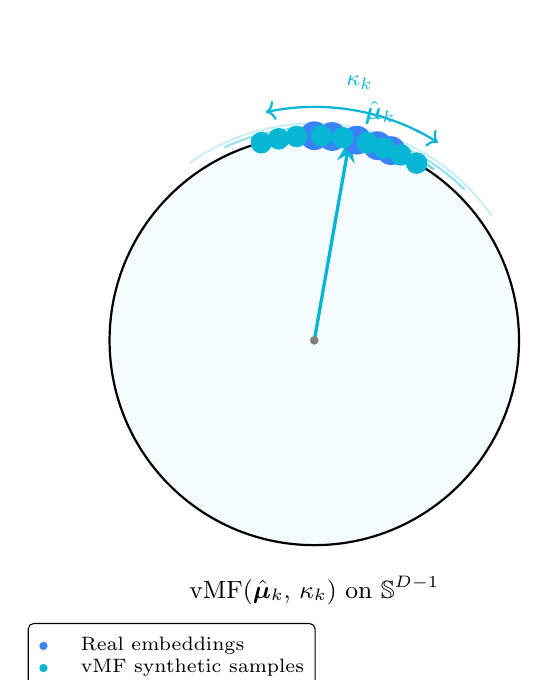
\begin{tikzpicture}[scale=2.6]
  %% Draw unit circle with subtle fill
  \draw[thick, fill=vmfcyan!4] (0,0) circle (1cm);

  %% Concentration density bands (wider = lower probability)
  \draw[vmfcyan!20, thick, domain=35:125, samples=60]
    plot ({1.06*cos(\x)},{1.06*sin(\x)});
  \draw[vmfcyan!40, thick, domain=45:115, samples=60]
    plot ({1.04*cos(\x)},{1.04*sin(\x)});
  \draw[vmfcyan!60, thick, domain=55:105, samples=60]
    plot ({1.02*cos(\x)},{1.02*sin(\x)});

  %% Mean direction arrow
  \draw[very thick, -Stealth, vmfcyan] (0,0) -- ({cos(80)},{sin(80)})
    node[above right=2pt, font=\small\bfseries]{$\hat{\bmu}_k$};

  %% Real embeddings (class k) — blue filled circles
  \foreach \a in {68,72,78,85,90} {
    \fill[encoderblue] ({cos(\a)},{sin(\a)}) circle (2pt);
  }

  %% vMF synthetic samples — cyan open circles with fill
  \foreach \a in {60,65,70,75,82,88,95,100,105} {
    \fill[vmfcyan] ({cos(\a)},{sin(\a)}) circle (1.5pt);
  }

  %% Kappa annotation arc
  \draw[<->, vmfcyan, thick] ({1.14*cos(58)},{1.14*sin(58)})
    arc (58:102:1.14);
  \node[vmfcyan, font=\footnotesize\bfseries]
    at ({1.28*cos(80)},{1.28*sin(80)}) {$\kappa_k$};

  %% Label below circle
  \node[font=\small] at (0,-1.22)
    {$\text{vMF}(\hat{\bmu}_k,\, \kappa_k)$ on $\Sphere^{D-1}$};

  %% Legend box
  \node[draw, rounded corners=2pt, fill=white, inner sep=4pt,
        font=\scriptsize, anchor=north west] at (-1.4, -1.38) {%
    \begin{tabular}{@{}cl@{}}
      \tikz\fill[encoderblue] (0,0) circle (1.5pt); & Real embeddings \\
      \tikz\fill[vmfcyan] (0,0) circle (1.5pt); & vMF synthetic samples \\
    \end{tabular}
  };

  %% Origin
  \fill[gray] (0,0) circle (0.6pt);
\end{tikzpicture}
\caption{Von~Mises--Fisher distributional sampling on the unit hypersphere.
A vMF distribution is fitted to each class's real embeddings (blue dots).
Synthetic samples (cyan dots) are drawn from the fitted distribution using
Wood's rejection algorithm.  Concentric arcs illustrate the probability
density contours; the concentration $\kappa_k$ controls the spread around
the class mean direction $\hat{\bmu}_k$.}
\label{fig:vmf}
\end{figure}

%% ─── FIG 5: Encoder Architecture ────────────────────────────────────────────
\begin{figure}[H]
\centering
\resizebox{0.92\textwidth}{!}{%
\begin{tikzpicture}[
  block/.style={draw, rectangle, rounded corners=3pt,
                minimum width=2cm, minimum height=0.7cm,
                font=\footnotesize\bfseries, align=center, thick},
  arr/.style={-Stealth, thick},
  node distance=0.6cm
]
  \node[block, fill=encoderblue!10, draw=encoderblue] (input)
    {Input\\$\bx \in \RR^{H \times W \times C}$};
  \node[block, fill=encoderblue!15, draw=encoderblue, right=0.8cm of input] (res1)
    {ResBlock Group 1\\{\scriptsize $64$ ch, $H/8$}};
  \node[block, fill=encoderblue!20, draw=encoderblue, right=0.8cm of res1] (res2)
    {ResBlock Group 2\\{\scriptsize $128$ ch, $H/16$}};
  \node[block, fill=encoderblue!25, draw=encoderblue, right=0.8cm of res2] (res3)
    {ResBlock Group 3\\{\scriptsize $256$ ch, $H/32$}};
  \node[block, fill=encoderblue!30, draw=encoderblue, right=0.8cm of res3] (res4)
    {ResBlock Group 4\\{\scriptsize $512$ ch, $H/64$}};
  \node[block, fill=gray!10, draw=gray, right=0.8cm of res4] (gap)
    {Global Avg Pool\\{\scriptsize $\mathbf{h} \in \RR^{512}$}};
  \node[block, fill=sngold!15, draw=sngold, right=0.8cm of gap] (proj)
    {Linear Proj.\\{\scriptsize $\mathbf{W}_{\text{proj}} \in \RR^{D \times 512}$}};
  \node[block, fill=slerpgreen!20, draw=slerpgreen, right=0.8cm of proj] (l2)
    {L2 Norm\\{\scriptsize $\bz = \mathbf{p}/\|\mathbf{p}\|_2$}};
  \node[block, fill=slerpgreen!30, draw=slerpgreen, right=0.8cm of l2] (out)
    {$\bz \in \Sphere^{D-1}$};

  \draw[arr] (input) -- (res1);
  \draw[arr] (res1) -- (res2);
  \draw[arr] (res2) -- (res3);
  \draw[arr] (res3) -- (res4);
  \draw[arr] (res4) -- (gap);
  \draw[arr] (gap) -- (proj);
  \draw[arr] (proj) -- (l2);
  \draw[arr] (l2) -- (out);

  %% Brace for "ResNet-18 Backbone (ImageNet pretrained)"
  \draw[decorate, decoration={brace, amplitude=6pt, mirror},
        thick, encoderblue!60]
    (res1.south west) -- (res4.south east)
    node[midway, below=8pt, font=\scriptsize, encoderblue]
    {ResNet-18 Backbone (ImageNet pretrained)};

  %% Brace for "L2 Normalization Head"
  \draw[decorate, decoration={brace, amplitude=6pt, mirror},
        thick, slerpgreen!60]
    (proj.south west) -- (l2.south east)
    node[midway, below=8pt, font=\scriptsize, slerpgreen]
    {L2 Normalization Head};
\end{tikzpicture}%
}%
\caption{Detailed encoder architecture (FIG.~3).  The ResNet-18 backbone
extracts a 512-dimensional feature vector, which is linearly projected and
L2-normalized to produce a unit-norm embedding $\bz \in \Sphere^{D-1}$.}
\label{fig:encoder}
\end{figure}

%% ─── FIG 6: Decoder Architecture ───────────────────────────────────────────
\begin{figure}[H]
\centering
\resizebox{0.92\textwidth}{!}{%
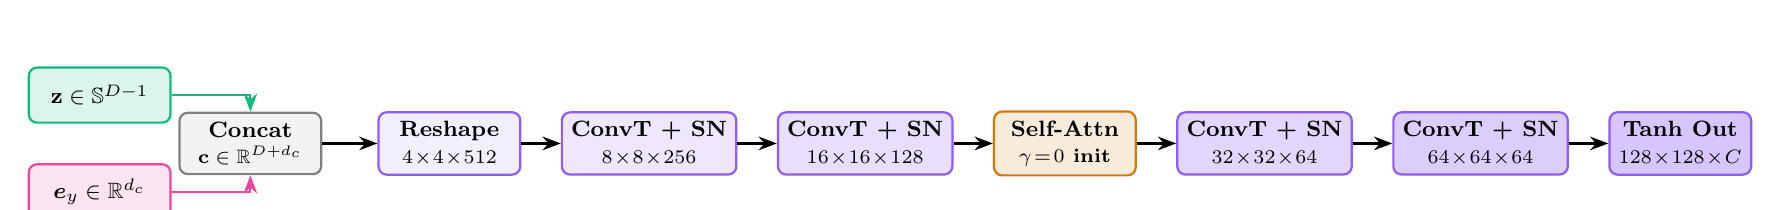
\begin{tikzpicture}[
  block/.style={draw, rectangle, rounded corners=3pt,
                minimum width=1.8cm, minimum height=0.7cm,
                font=\footnotesize\bfseries, align=center, thick},
  arr/.style={-Stealth, thick},
  node distance=0.5cm
]
  %% Inputs
  \node[block, fill=slerpgreen!15, draw=slerpgreen] (zin)
    {$\bz \in \Sphere^{D-1}$};
  \node[block, fill=projmagenta!15, draw=projmagenta, below=0.5cm of zin] (ein)
    {$\bm{e}_y \in \RR^{d_c}$};

  %% Concatenation
  \node[block, fill=gray!10, draw=gray, right=1cm of $(zin)!0.5!(ein)$] (concat)
    {Concat\\{\scriptsize $\bc \in \RR^{D+d_c}$}};

  %% Decoder blocks
  \node[block, fill=decoderviolet!10, draw=decoderviolet, right=0.7cm of concat] (reshape)
    {Reshape\\{\scriptsize $4\!\times\!4\!\times\!512$}};
  \node[block, fill=decoderviolet!15, draw=decoderviolet, right=0.5cm of reshape] (ct1)
    {ConvT + SN\\{\scriptsize $8\!\times\!8\!\times\!256$}};
  \node[block, fill=decoderviolet!20, draw=decoderviolet, right=0.5cm of ct1] (ct2)
    {ConvT + SN\\{\scriptsize $16\!\times\!16\!\times\!128$}};
  \node[block, fill=sngold!15, draw=sngold, right=0.5cm of ct2] (attn)
    {Self-Attn\\{\scriptsize $\gamma\!=\!0$ init}};
  \node[block, fill=decoderviolet!25, draw=decoderviolet, right=0.5cm of attn] (ct3)
    {ConvT + SN\\{\scriptsize $32\!\times\!32\!\times\!64$}};
  \node[block, fill=decoderviolet!30, draw=decoderviolet, right=0.5cm of ct3] (ct4)
    {ConvT + SN\\{\scriptsize $64\!\times\!64\!\times\!64$}};
  \node[block, fill=decoderviolet!35, draw=decoderviolet, right=0.5cm of ct4] (ct5)
    {Tanh Out\\{\scriptsize $128\!\times\!128\!\times\!C$}};

  %% Arrows
  \draw[arr, slerpgreen] (zin.east) -| (concat.north);
  \draw[arr, projmagenta] (ein.east) -| (concat.south);
  \draw[arr] (concat) -- (reshape);
  \draw[arr] (reshape) -- (ct1);
  \draw[arr] (ct1) -- (ct2);
  \draw[arr] (ct2) -- (attn);
  \draw[arr] (attn) -- (ct3);
  \draw[arr] (ct3) -- (ct4);
  \draw[arr] (ct4) -- (ct5);
\end{tikzpicture}%
}%
\caption{Class-conditional DCGAN decoder architecture (FIG.~6).  The image
embedding $\bz$ and class embedding $\bm{e}_y$ are concatenated, then
progressively upsampled through spectrally normalised transposed convolutions.
A non-local self-attention block at $16\!\times\!16$ resolution captures
long-range spatial dependencies.}
\label{fig:decoder}
\end{figure}

%% ─── FIG 7: Projection Discriminator ───────────────────────────────────────
\begin{figure}[H]
\centering
\resizebox{0.88\textwidth}{!}{%
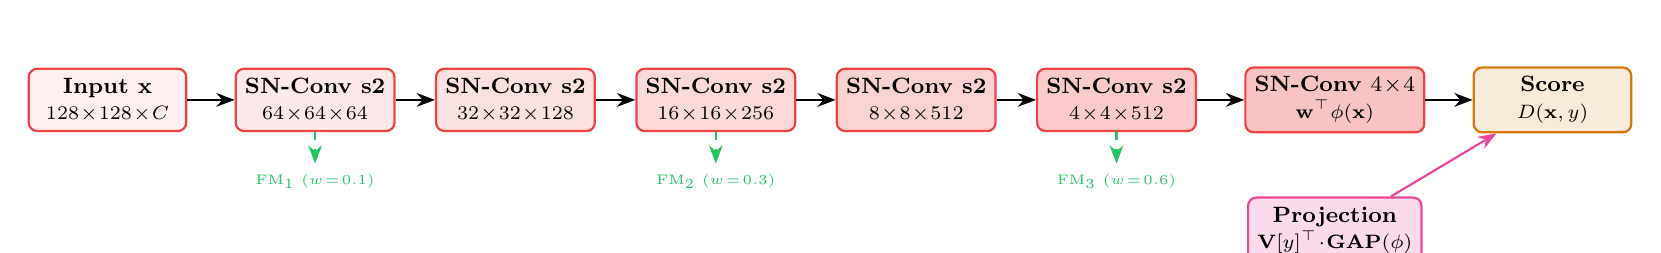
\begin{tikzpicture}[
  block/.style={draw, rectangle, rounded corners=3pt,
                minimum width=2cm, minimum height=0.7cm,
                font=\footnotesize\bfseries, align=center, thick},
  arr/.style={-Stealth, thick},
  node distance=0.5cm
]
  %% Input
  \node[block, fill=discrimred!8, draw=discrimred] (inp)
    {Input $\bx$\\{\scriptsize $128\!\times\!128\!\times\!C$}};

  %% Conv blocks
  \node[block, fill=discrimred!12, draw=discrimred, right=0.6cm of inp] (c1)
    {SN-Conv s2\\{\scriptsize $64\!\times\!64\!\times\!64$}};
  \node[block, fill=discrimred!16, draw=discrimred, right=0.5cm of c1] (c2)
    {SN-Conv s2\\{\scriptsize $32\!\times\!32\!\times\!128$}};
  \node[block, fill=discrimred!20, draw=discrimred, right=0.5cm of c2] (c3)
    {SN-Conv s2\\{\scriptsize $16\!\times\!16\!\times\!256$}};
  \node[block, fill=discrimred!24, draw=discrimred, right=0.5cm of c3] (c4)
    {SN-Conv s2\\{\scriptsize $8\!\times\!8\!\times\!512$}};
  \node[block, fill=discrimred!28, draw=discrimred, right=0.5cm of c4] (c5)
    {SN-Conv s2\\{\scriptsize $4\!\times\!4\!\times\!512$}};

  %% Final + projection
  \node[block, fill=discrimred!32, draw=discrimred, right=0.6cm of c5] (final)
    {SN-Conv $4\!\times\!4$\\{\scriptsize $\bw^\top\phi(\bx)$}};

  \node[block, fill=projmagenta!20, draw=projmagenta, below=0.8cm of final] (proj)
    {Projection\\{\scriptsize $\mathbf{V}[y]^\top\!\cdot\!\text{GAP}(\phi)$}};

  \node[block, fill=sngold!15, draw=sngold, right=0.6cm of final] (score)
    {Score\\{\scriptsize $D(\bx, y)$}};

  %% Arrows
  \draw[arr] (inp) -- (c1);
  \draw[arr] (c1) -- (c2);
  \draw[arr] (c2) -- (c3);
  \draw[arr] (c3) -- (c4);
  \draw[arr] (c4) -- (c5);
  \draw[arr] (c5) -- (final);
  \draw[arr] (final) -- (score);
  \draw[arr, projmagenta] (proj) -- (score);

  %% Feature extraction markers
  \draw[-Stealth, phasegreen, thick, dashed] (c1.south) -- ++(0,-0.4)
    node[below, font=\tiny, phasegreen]{FM$_1$ ($w\!=\!0.1$)};
  \draw[-Stealth, phasegreen, thick, dashed] (c3.south) -- ++(0,-0.4)
    node[below, font=\tiny, phasegreen]{FM$_2$ ($w\!=\!0.3$)};
  \draw[-Stealth, phasegreen, thick, dashed] (c5.south) -- ++(0,-0.4)
    node[below, font=\tiny, phasegreen]{FM$_3$ ($w\!=\!0.6$)};
\end{tikzpicture}%
}%
\caption{Projection discriminator architecture (FIG.~8).  All Conv2d layers
use spectral normalisation (SN).  Feature maps are extracted at three depths
for multi-scale feature matching (dashed green arrows).  The projection head
computes a class-conditional bias via
$\mathbf{V}[y]^\top\!\cdot\!\text{GAP}(\phi(\bx))$.}
\label{fig:disc}
\end{figure}

%% ─── FIG 8: Adaptive Lambda Controller ─────────────────────────────────────
\begin{figure}[H]
\centering
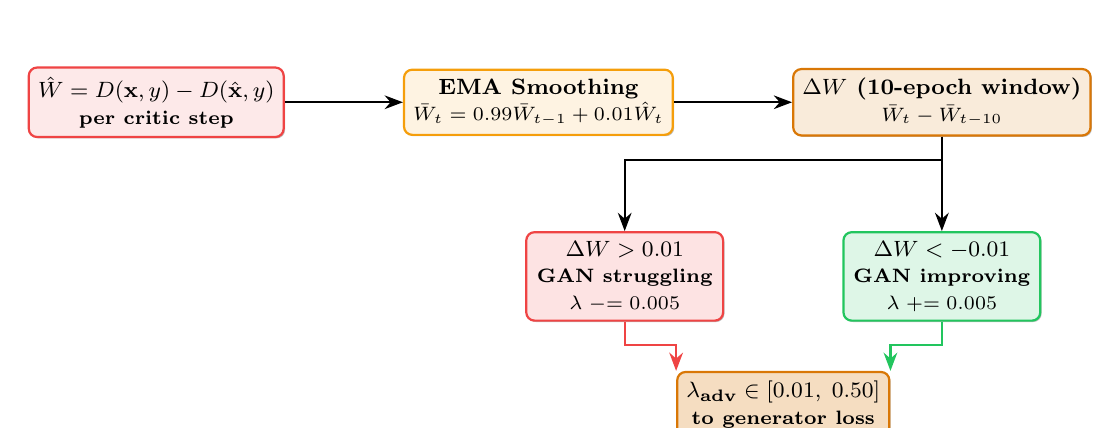
\begin{tikzpicture}[
  block/.style={draw, rectangle, rounded corners=3pt,
                minimum width=2.5cm, minimum height=0.8cm,
                font=\footnotesize\bfseries, align=center, thick,
                drop shadow={shadow xshift=0.5pt, shadow yshift=-0.5pt}},
  arr/.style={-Stealth, thick},
  node distance=0.8cm
]
  %% Components
  \node[block, fill=discrimred!12, draw=discrimred] (west)
    {$\hat{W} = D(\bx,y) - D(\hat{\bx},y)$\\{\scriptsize per critic step}};

  \node[block, fill=emaorange!12, draw=emaorange, right=1.5cm of west] (ema)
    {EMA Smoothing\\{\scriptsize $\bar{W}_t = 0.99\bar{W}_{t-1} + 0.01\hat{W}_t$}};

  \node[block, fill=sngold!15, draw=sngold, right=1.5cm of ema] (delta)
    {$\Delta W$ (10-epoch window)\\{\scriptsize $\bar{W}_t - \bar{W}_{t-10}$}};

  \node[block, fill=phasegreen!15, draw=phasegreen, below=1.2cm of delta] (inc)
    {$\Delta W < -0.01$\\{\scriptsize GAN improving}\\{\scriptsize $\lambda \mathrel{+}= 0.005$}};

  \node[block, fill=discrimred!15, draw=discrimred, left=1.5cm of inc] (dec)
    {$\Delta W > 0.01$\\{\scriptsize GAN struggling}\\{\scriptsize $\lambda \mathrel{-}= 0.005$}};

  \node[block, fill=sngold!25, draw=sngold, below=1.2cm of $(dec)!0.5!(inc)$] (output)
    {$\lambda_{\text{adv}} \in [0.01,\; 0.50]$\\{\scriptsize to generator loss}};

  %% Arrows
  \draw[arr] (west) -- (ema);
  \draw[arr] (ema) -- (delta);
  \draw[arr] (delta.south) -- ++(0,-0.3) -| (inc.north);
  \draw[arr] (delta.south) -- ++(0,-0.3) -| (dec.north);
  \draw[arr, phasegreen] (inc.south) -- ++(0,-0.3) -| (output.north east);
  \draw[arr, discrimred] (dec.south) -- ++(0,-0.3) -| (output.north west);

\end{tikzpicture}
\caption{Adaptive adversarial loss weight controller (FIG.~10).  The
Wasserstein distance estimate is EMA-smoothed and monitored over a
10-epoch sliding window.  The adversarial weight $\lambda_{\text{adv}}$
increases when the GAN is improving (decreasing $W$-distance) and decreases
when struggling (increasing $W$-distance), bounded within $[0.01, 0.50]$.}
\label{fig:adaptive_lambda}
\end{figure}

%% ─── FIG 9: Complete Synthesis Flow ────────────────────────────────────────
\begin{figure}[H]
\centering
\begin{tikzpicture}[
  step/.style={draw, rectangle, rounded corners=3pt,
               minimum width=3.5cm, minimum height=0.8cm,
               font=\footnotesize\bfseries, align=center, thick},
  decision/.style={draw, diamond, aspect=2.5,
                   minimum width=2.5cm,
                   font=\footnotesize\bfseries, align=center, thick},
  arr/.style={-Stealth, thick},
  node distance=0.9cm
]
  \node[step, fill=encoderblue!12, draw=encoderblue] (load)
    {Load Dataset\\{\scriptsize (Universal Interface)}};

  \node[step, fill=encoderblue!20, draw=encoderblue, below=0.7cm of load] (encode)
    {Encode All Images\\{\scriptsize $\bz_i = E_{\tilde{\bphi}}(\bx_i)$}};

  \node[step, fill=gray!10, draw=gray, below=0.7cm of encode] (identify)
    {Identify Minority Classes\\{\scriptsize $n_c < N_{\text{target}}$}};

  \node[decision, fill=slerpgreen!10, draw=slerpgreen, below=0.8cm of identify] (mode)
    {Mode?};

  \node[step, fill=slerpgreen!20, draw=slerpgreen, below left=1cm and 1cm of mode] (slerp)
    {SLERP-SMOTE\\{\scriptsize $k$-NN + geodesic arc}};

  \node[step, fill=vmfcyan!20, draw=vmfcyan, below right=1cm and 1cm of mode] (vmf)
    {vMF-SMOTE\\{\scriptsize Fit + Wood's sample}};

  \node[step, fill=decoderviolet!15, draw=decoderviolet, below=1.5cm of mode] (decode)
    {Decode Synthetic Embeddings\\{\scriptsize $\hat{\bx} = G_{\tilde{\btheta}}([\hat{\bz};\, \bm{e}_c])$}};

  \node[step, fill=phasegreen!15, draw=phasegreen, below=0.7cm of decode] (output)
    {Augmented Dataset\\{\scriptsize Real + Synthetic Images}};

  %% Arrows
  \draw[arr] (load) -- (encode);
  \draw[arr] (encode) -- (identify);
  \draw[arr] (identify) -- (mode);
  \draw[arr, slerpgreen] (mode) -- node[left, font=\scriptsize]{slerp} (slerp);
  \draw[arr, vmfcyan] (mode) -- node[right, font=\scriptsize]{vmf} (vmf);
  \draw[arr, slerpgreen] (slerp) |- (decode);
  \draw[arr, vmfcyan] (vmf) |- (decode);
  \draw[arr] (decode) -- (output);

\end{tikzpicture}
\caption{Complete synthetic image generation procedure (FIG.~13).  After
training, the system encodes all images, identifies minority classes,
synthesizes new embeddings via either SLERP or vMF mode, and decodes them
through the EMA-weight decoder to produce the augmented dataset.}
\label{fig:synthesis_flow}
\end{figure}

%% ─── FIG 10: EMA Manager ──────────────────────────────────────────────────
\begin{figure}[H]
\centering
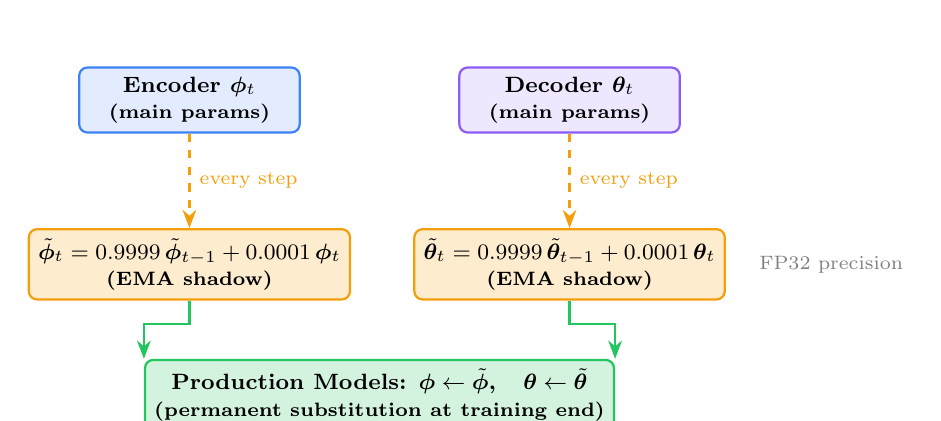
\begin{tikzpicture}[
  block/.style={draw, rectangle, rounded corners=3pt,
                minimum width=2.8cm, minimum height=0.7cm,
                font=\footnotesize\bfseries, align=center, thick},
  arr/.style={-Stealth, thick},
  dasharr/.style={-Stealth, thick, dashed},
  node distance=0.6cm
]
  %% Training parameters
  \node[block, fill=encoderblue!15, draw=encoderblue] (enc_main)
    {Encoder $\bphi_t$\\{\scriptsize (main params)}};
  \node[block, fill=decoderviolet!15, draw=decoderviolet, right=2cm of enc_main] (dec_main)
    {Decoder $\btheta_t$\\{\scriptsize (main params)}};

  %% EMA shadow
  \node[block, fill=emaorange!20, draw=emaorange, below=1.2cm of enc_main] (enc_ema)
    {$\tilde{\bphi}_t = 0.9999\,\tilde{\bphi}_{t-1} + 0.0001\,\bphi_t$\\{\scriptsize (EMA shadow)}};
  \node[block, fill=emaorange!20, draw=emaorange, below=1.2cm of dec_main] (dec_ema)
    {$\tilde{\btheta}_t = 0.9999\,\tilde{\btheta}_{t-1} + 0.0001\,\btheta_t$\\{\scriptsize (EMA shadow)}};

  %% Production models
  \node[block, fill=phasegreen!20, draw=phasegreen, below=1.2cm of $(enc_ema)!0.5!(dec_ema)$] (prod)
    {Production Models: $\bphi \leftarrow \tilde{\bphi}$,\quad $\btheta \leftarrow \tilde{\btheta}$\\{\scriptsize (permanent substitution at training end)}};

  %% Arrows
  \draw[dasharr, emaorange] (enc_main) -- (enc_ema)
    node[midway, right, font=\scriptsize]{every step};
  \draw[dasharr, emaorange] (dec_main) -- (dec_ema)
    node[midway, right, font=\scriptsize]{every step};
  \draw[arr, phasegreen] (enc_ema.south) -- ++(0,-0.3) -| (prod.north west);
  \draw[arr, phasegreen] (dec_ema.south) -- ++(0,-0.3) -| (prod.north east);

  %% FP32 annotation
  \node[font=\scriptsize, gray, right=0.3cm of dec_ema]
    {FP32 precision};
\end{tikzpicture}
\caption{EMA shadow parameter manager (FIG.~11).  Shadow parameters are
maintained at FP32 precision for both encoder and decoder, updated after
every gradient step with decay $\mu = 0.9999$, and permanently substituted
into the production models at training completion.}
\label{fig:ema}
\end{figure}

% ══════════════════════════════════════════════════════════════════════════════
%  ALGORITHM PSEUDOCODE
% ══════════════════════════════════════════════════════════════════════════════

\subsection{Algorithm Pseudocode}

\begin{algorithm}[H]
\caption{Dual-Mode Oversampling (Inference)}
\label{alg:oversample}
\begin{algorithmic}[1]
\Require Trained encoder $E_{\tilde{\bphi}}$, EMA decoder $G_{\tilde{\btheta}}$,
         training images $\{\bx_i, y_i\}_{i=1}^N$, target count $N_{\text{target}}$,
         mode $\in \{\texttt{slerp},\, \texttt{vmf}\}$, neighbors $k=5$
\State Compute embeddings: $\bz_i \leftarrow E_{\tilde{\bphi}}(\bx_i)$ for all $i$
\For{each class $c$ with $n_c < N_{\text{target}}$}
  \State $\mathcal{Z}_c \leftarrow \{\bz_i : y_i = c\}$;\quad
         $n_{\text{syn}} \leftarrow N_{\text{target}} - n_c$
  \If{mode = \texttt{vmf}}
    \State $\hat{\bmu}_c, \hat{\kappa}_c \leftarrow
      \textsc{MLE-vMF}(\mathcal{Z}_c)$
      \Comment{Eq.~(\ref{eq:kappa_mle})}
    \State $\kappa_c \leftarrow s \cdot \hat{\kappa}_c$
      \Comment{User-specified scale $s$}
    \For{$j = 1$ to $n_{\text{syn}}$}
      \State $\hat{\bz}_j \leftarrow \textsc{Wood-Sample}
        (\hat{\bmu}_c,\, \kappa_c)$
        \Comment{Unit-norm by construction}
    \EndFor
  \Else \Comment{mode = \texttt{slerp}}
    \For{$j = 1$ to $n_{\text{syn}}$}
      \State Sample anchor $\bz_0 \sim \mathcal{Z}_c$ uniformly
      \State $\bz_1 \leftarrow k\text{-NN}(\bz_0,\, \mathcal{Z}_c)$
        \Comment{Cosine similarity}
      \State $\omega \leftarrow \arccos(\bz_0 \cdot \bz_1)$
      \State $t \sim \text{Uniform}(0,1)$
      \If{$\omega < 10^{-6}$}
        $\hat{\bz}_j \leftarrow \text{normalize}((1-t)\bz_0 + t\bz_1)$
      \Else\
        $\hat{\bz}_j \leftarrow \text{SLERP}(\bz_0, \bz_1, t)$
        \Comment{Eq.~(\ref{eq:slerp})}
      \EndIf
    \EndFor
  \EndIf
  \State $\bm{e}_c \leftarrow \mathbf{E}_c[c]$
  \For{each $\hat{\bz}_j$}
    \State $\hat{\bx}_j \leftarrow G_{\tilde{\btheta}}
      ([\hat{\bz}_j;\, \bm{e}_c])$
    \State Add $(\hat{\bx}_j, c)$ to augmented corpus
  \EndFor
\EndFor
\end{algorithmic}
\end{algorithm}

\begin{algorithm}[H]
\caption{End-to-End Training with Adaptive Adversarial Dynamics}
\label{alg:train}
\begin{algorithmic}[1]
\Require Dataset $\mathcal{D}$, total epochs $T$, phase boundary $\tau = 0.3T$
\State Init $E_{\bphi}$, $G_{\btheta}$, projection disc.\ $D_{\bpsi}$ (with SN)
\State Init EMA: $\tilde{\btheta} \leftarrow \btheta$,
  $\tilde{\bphi} \leftarrow \bphi$
\State Init $\lambda_{\text{adv}} \leftarrow 0.05$,
  $\bar{W} \leftarrow 0$, window $\leftarrow []$
\For{epoch $t = 0$ to $T-1$}
  \For{each minibatch $(\bx, y) \sim \mathcal{D}$}
    \State $\bz \leftarrow E_{\bphi}(\bx)$;\quad
      $\hat{\bx} \leftarrow G_{\btheta}([\bz;\, \mathbf{E}_c[y]])$
    \State $\mathcal{L} \leftarrow \mathcal{L}_{\text{recon}}(\bx, \hat{\bx})$
      \Comment{MSE + L1 + Perceptual}
    \If{$t \geq \tau$} \Comment{Phase 2}
      \For{$n = 1$ to $5$}
        \State Update $D_{\bpsi}$ with $\mathcal{L}_D$
          (SN + GP, projection scoring)
        \State $\hat{W} \leftarrow D_{\bpsi}(\bx,y) - D_{\bpsi}(\hat{\bx},y)$
      \EndFor
      \State $\mathcal{L} \mathrel{+}= \lambda_{\text{adv}}\mathcal{L}_G
        + 0.1\,\mathcal{L}_{\text{FM}} + \lambda_r\,\mathcal{L}_{\text{repulse}}$
    \EndIf
    \State Update $E_{\bphi}, G_{\btheta}$ with
      $\nabla \mathcal{L}$ (clip grad norm $\leq 1.0$)
    \State $\tilde{\btheta} \leftarrow 0.9999\,\tilde{\btheta}
      + 0.0001\,\btheta$;\quad
      $\tilde{\bphi} \leftarrow 0.9999\,\tilde{\bphi}
      + 0.0001\,\bphi$
  \EndFor
  \If{$t \geq \tau$}
    \State Update $\bar{W}$, compute $\Delta W$ over 10-epoch window
    \State Adjust $\lambda_{\text{adv}}$ via feedback rule
  \EndIf
  \State Step cosine LR schedulers; save checkpoint
\EndFor
\State $\btheta \leftarrow \tilde{\btheta}$;\quad
  $\bphi \leftarrow \tilde{\bphi}$
  \Comment{Permanent EMA substitution}
\end{algorithmic}
\end{algorithm}

\subsection{Quality Assessment Metrics}

\subsubsection{Fr\'{e}chet Inception Distance}

The primary metric is the FID~\cite{heusel2017}:

\begin{equation}
  \text{FID} = \|\bmu_r - \bmu_s\|_2^2
    + \text{tr}\!\left(\bm{\Sigma}_r + \bm{\Sigma}_s
      - 2\bigl(\bm{\Sigma}_r \bm{\Sigma}_s\bigr)^{1/2}\right),
  \label{eq:fid}
\end{equation}

where $(\bmu_r, \bm{\Sigma}_r)$ and $(\bmu_s, \bm{\Sigma}_s)$ denote the
mean and covariance of Inception-v3 features for real and synthetic images.
Intra-class FID is also computed per class.  Downstream classifier
performance (per-class recall, F1, AUROC) provides the ultimate utility
measure.

% ══════════════════════════════════════════════════════════════════════════════
\newpage
\section*{CLAIMS}
% ══════════════════════════════════════════════════════════════════════════════

What is claimed is:

\begin{claims}

%% ── Method Claims (1–25) ────────────────────────────────────────────────────

\item A computer-implemented method for generating class-conditional synthetic
images to address class imbalance in an image dataset, the method comprising:
\begin{enumerate}[label=(\alph*),leftmargin=1.5em,nosep]
  \item receiving, by a processing system, an image dataset comprising a
    plurality of images organized by class label, wherein at least one class
    is underrepresented relative to at least one other class;
  \item encoding, by a convolutional neural network encoder augmented with an
    L2~normalization head, each image to a unit-norm embedding vector on a
    unit hypersphere $\Sphere^{D-1}$;
  \item constructing, for each underrepresented class, one or more synthetic
    embedding vectors by at least one of:
    \begin{enumerate}[label=(\roman*),nosep]
      \item spherical linear interpolation (SLERP) along a geodesic arc of
        $\Sphere^{D-1}$ connecting a first same-class unit-norm embedding
        vector and a second same-class unit-norm embedding vector; or
      \item sampling from a von~Mises--Fisher (vMF) distribution fitted to
        the unit-norm embeddings of the underrepresented class;
    \end{enumerate}
  \item forming a conditioning vector by concatenating each synthetic
    embedding vector with a learned class embedding vector; and
  \item generating, by a class-conditional convolutional decoder receiving
    the conditioning vector, a synthetic image for the underrepresented class.
\end{enumerate}

\item The method of claim~1, wherein the SLERP is computed according to
$\hat{\bz}(t) = \frac{\sin((1-t)\omega)}{\sin\omega}\bz_0 +
\frac{\sin(t\omega)}{\sin\omega}\bz_1$, where $\omega =
\arccos(\bz_0 \cdot \bz_1)$ and $t \sim \text{Uniform}(0,1)$.

\item The method of claim~2, further comprising detecting when $\omega <
\epsilon$ and computing the synthetic embedding as the L2~normalization of
$(1-t)\bz_0 + t\bz_1$.

\item The method of claim~1, wherein the vMF distribution parameters are
estimated by maximum likelihood, with mean direction
$\hat{\bmu} = \bar{\bz}/\|\bar{\bz}\|_2$ and concentration
$\hat{\kappa} \approx \bar{R}(D - \bar{R}^2)/(1 - \bar{R}^2)$ where
$\bar{R} = \|\bar{\bz}\|_2$.

\item The method of claim~4, further comprising applying a user-configurable
concentration scale factor $s > 0$ to the MLE-estimated concentration,
yielding $\kappa = s \cdot \hat{\kappa}$.

\item The method of claim~4, wherein synthetic embeddings are sampled from
the vMF distribution using Wood's rejection algorithm with Householder
reflection.

\item The method of claim~1, wherein the second same-class embedding is
selected from a set of $k$ nearest neighbors determined by cosine similarity,
with $k = 5$ in the preferred embodiment.

\item The method of claim~7, wherein the $k$-nearest-neighbor selection is
constrained to within-cluster neighbors, preventing interpolation between
semantically distant modes of the same class.

\item The method of claim~1, wherein the class-conditional convolutional
decoder comprises transposed convolutional layers with spectral
normalisation and a non-local self-attention block at $16 \times 16$
spatial resolution with a zero-initialized output scale parameter
$\gamma_{\text{attn}}$.

\item The method of claim~1, further comprising discriminating real from
synthesized images using a projection discriminator that computes a
class-conditional critic score as
$D(\bx, y) = \bw^\top\phi(\bx) + \mathbf{V}[y]^\top\text{GAP}(\phi(\bx))$,
wherein $\mathbf{V}$ is a learned class embedding table.

\item The method of claim~10, wherein every convolutional layer of the
projection discriminator is wrapped with spectral normalisation.

\item The method of claim~1, further comprising jointly training the encoder,
decoder, and discriminator using a phased schedule comprising:
\begin{enumerate}[label=(\roman*),nosep]
  \item a first phase using only a reconstruction loss; and
  \item a second phase using a Wasserstein GAN loss with gradient penalty,
    multi-scale feature matching loss, and intra-class diversity repulsion
    loss, with adaptive adversarial loss weighting.
\end{enumerate}

\item The method of claim~12, wherein the adaptive adversarial loss weight
$\lambda_{\text{adv}}$ is adjusted based on an EMA-smoothed Wasserstein
distance monitor, increasing when the Wasserstein distance is decreasing and
decreasing when the Wasserstein distance is increasing.

\item The method of claim~13, wherein $\lambda_{\text{adv}}$ is bounded
within $[0.01,\, 0.50]$ and follows a linear ramp during initial warmup
before the feedback mechanism activates.

\item The method of claim~12, wherein the multi-scale feature matching loss
comprises L1 discrepancies at three discriminator depths with progressive
weights $(0.1, 0.3, 0.6)$.

\item The method of claim~12, wherein the intra-class diversity repulsion
loss penalizes excessive cosine similarity between embeddings of the same
class within each minibatch using a hinge margin.

\item The method of claim~12, further comprising maintaining exponential
moving average shadow parameters of both the encoder and the decoder,
updated after each gradient step with decay $\mu = 0.9999$, and permanently
substituting the shadow parameters upon training completion.

\item The method of claim~12, wherein the reconstruction loss comprises a
pixel-level MSE term, a pixel-level L1 term, and a perceptual loss computed
in the feature space of a pretrained VGG-16 network.

\item The method of claim~1, wherein the learned class embedding vector has
dimensionality $d_c = 64$ and is drawn from a class embedding matrix
$\mathbf{E}_c \in \RR^{K \times 64}$ jointly trained with the encoder and
decoder.

\item The method of claim~1, further comprising loading the image dataset
using a universal dataset interface that automatically discovers class labels
by enumerating subdirectories without dataset-specific configuration.

\item The method of claim~1, further comprising applying outlier detection
to synthetic embeddings and resampling rejected outliers.

\item The method of claim~1, further comprising recording provenance
metadata for each synthetic sample including parent indices, interpolation
parameter, synthesis method, and cluster assignment.

\item The method of claim~2, wherein the interpolation parameter $t$ is
density-weighted, biased toward $0.5$ in low-density geodesic regions and
drawn uniformly in high-density regions.

%% ── System Claims (24–32) ───────────────────────────────────────────────────

\item A system for generating class-conditional synthetic images to address
class imbalance in an image dataset, the system comprising:
a processor and a non-transitory computer-readable memory storing
instructions that, when executed, configure the processor to implement:
\begin{enumerate}[label=(\alph*),leftmargin=1.5em,nosep]
  \item a convolutional encoder with an L2~normalization head mapping input
    images to unit-norm embeddings on $\Sphere^{D-1}$;
  \item a dual-mode oversampling module supporting both SLERP interpolation
    along class-homogeneous geodesic arcs and von~Mises--Fisher distributional
    sampling from per-class fitted distributions;
  \item a class-conditional convolutional decoder with a learned class
    embedding lookup, transposed convolutional layers with spectral
    normalisation, and a non-local self-attention block;
  \item a projection discriminator with spectral normalisation on all
    convolutional layers and a class-conditional projection scoring
    mechanism; and
  \item an adaptive adversarial loss weight controller that adjusts
    $\lambda_{\text{adv}}$ based on EMA-smoothed Wasserstein distance
    monitoring.
\end{enumerate}

\item The system of claim~24, further comprising an EMA manager maintaining
shadow parameters for both encoder and decoder with decay $\mu = 0.9999$,
and permanently substituting shadow parameters upon training completion.

\item The system of claim~24, further comprising a multi-scale feature
matching module extracting features at three discriminator depths with
progressive weights.

\item The system of claim~24, further comprising an intra-class diversity
repulsion loss module penalizing excessive within-class cosine similarity.

\item The system of claim~24, further comprising per-class outlier
detectors for filtering synthetic embeddings.

\item The system of claim~24, further comprising a universal dataset
interface that automatically discovers class labels from a folder hierarchy.

%% ── CRM Claims (30–33) ─────────────────────────────────────────────────────

\item A non-transitory computer-readable medium storing instructions that,
when executed by one or more processors, cause the processors to perform a
method comprising:
\begin{enumerate}[label=(\alph*),leftmargin=1.5em,nosep]
  \item encoding training images of underrepresented classes to unit-norm
    embeddings on $\Sphere^{D-1}$ using a convolutional encoder with an
    L2~normalization head;
  \item for each synthetic image to be generated, constructing a synthetic
    embedding by one of:
    \begin{enumerate}[label=(\roman*),nosep]
      \item SLERP along a geodesic arc connecting two same-class embeddings; or
      \item sampling from a vMF distribution fitted to the class embeddings;
    \end{enumerate}
  \item forming a decoder input by concatenating the synthetic embedding with
    a learned class embedding;
  \item decoding the input to a synthetic image using a class-conditional
    decoder with spectral normalisation and self-attention; and
  \item adding the synthetic image to a training corpus.
\end{enumerate}

\item The medium of claim~30, wherein the method further comprises training
using a phased schedule with adaptive adversarial loss weighting controlled
by an EMA-smoothed Wasserstein distance monitor.

\item The medium of claim~30, wherein the discriminator is a projection
discriminator computing
$D(\bx,y) = \bw^\top\phi(\bx) + \mathbf{V}[y]^\top\text{GAP}(\phi(\bx))$
with spectral normalisation on all convolutional layers.

%% ── Training Method Claims (33–35) ─────────────────────────────────────────

\item A method for training an adversarial image synthesis system for
class-conditional image oversampling, the method comprising:
\begin{enumerate}[label=(\alph*),leftmargin=1.5em,nosep]
  \item initializing a convolutional encoder with an L2~normalization head,
    a class-conditional DCGAN decoder with spectral normalisation, and a
    projection discriminator with spectral normalisation;
  \item in a first training phase, updating encoder and decoder parameters
    using only a reconstruction loss comprising MSE, L1, and perceptual
    loss terms;
  \item transitioning to a second phase at approximately thirty percent of
    total epochs, activating a Wasserstein GAN loss with gradient penalty,
    multi-scale feature matching loss, and intra-class repulsion loss;
  \item adaptively adjusting the adversarial loss weight
    $\lambda_{\text{adv}}$ via feedback from an EMA-smoothed Wasserstein
    distance monitor;
  \item maintaining EMA shadow parameters for both encoder and decoder
    throughout training; and
  \item upon completion, substituting the EMA shadow parameters and saving
    the resulting models.
\end{enumerate}

\item The method of claim~33, wherein $\lambda_{\text{adv}}$ increases by
$0.005$ per epoch when the smoothed Wasserstein distance decreases, and
decreases by $0.005$ when it increases, bounded within $[0.01,\; 0.50]$.

\item The method of claim~33, wherein gradient norms for the generator
parameters are clipped to a maximum of $1.0$.

\end{claims}

% ══════════════════════════════════════════════════════════════════════════════
\newpage
\section*{ABSTRACT}
% ══════════════════════════════════════════════════════════════════════════════

A system and method for generating photorealistic class-conditional synthetic
images to address class imbalance in image datasets.  A convolutional neural
network encoder, augmented with an L2~normalization head that projects
outputs onto a unit hypersphere $\Sphere^{D-1}$, maps training images to
unit-norm embedding vectors.  A dual-mode oversampling module synthesizes new
embedding vectors by either (a)~spherical linear interpolation (SLERP) along
geodesic arcs connecting $k$-nearest-neighbor pairs within each minority
class, preserving the unit-norm constraint and manifold fidelity; or
(b)~von~Mises--Fisher (vMF) distributional sampling fitted per class,
providing pair-selection-free coverage of the class distribution on the
hypersphere.  A class-conditional DCGAN decoder with non-local self-attention
at $16\times16$ resolution, spectral normalisation, and zero-initialized
$\gamma$ weighting decodes synthetic embeddings to images.  A projection
discriminator with spectral normalisation provides class-conditional
adversarial feedback.  Encoder, decoder, and discriminator are jointly trained
through a phased schedule: reconstruction-only for the first thirty percent of
epochs, followed by Wasserstein GAN training with gradient penalty,
multi-scale feature matching, and intra-class repulsion loss with adaptive
adversarial weighting controlled by an EMA-smoothed Wasserstein distance
monitor.  Exponential moving average shadow parameters ($\mu = 0.9999$) are
maintained for both encoder and decoder and permanently substituted
post-training.  A universal dataset interface ingests any folder-structured
image dataset.  The system generates class-faithful synthetic images that
demonstrably improve downstream classifier performance on class-imbalanced
datasets.

% ══════════════════════════════════════════════════════════════════════════════
\newpage
\begin{thebibliography}{99}

\bibitem{chawla2002}
N.~V.~Chawla, K.~W.~Bowyer, L.~O.~Hall, and W.~P.~Kegelmeyer,
``SMOTE: Synthetic Minority Over-sampling Technique,''
\textit{J.\ Artif.\ Intell.\ Res.}, vol.~16, pp.~321--357, 2002.

\bibitem{he2016}
K.~He, X.~Zhang, S.~Ren, and J.~Sun,
``Deep Residual Learning for Image Recognition,''
\textit{Proc.\ IEEE CVPR}, Las Vegas, NV, pp.~770--778, 2016.

\bibitem{radford2016}
A.~Radford, L.~Metz, and S.~Chintala,
``Unsupervised Representation Learning with Deep Convolutional Generative
Adversarial Networks,''
\textit{ICLR}, San Juan, PR, 2016.

\bibitem{gulrajani2017}
I.~Gulrajani, F.~Ahmed, M.~Arjovsky, V.~Dumoulin, and A.~Courville,
``Improved Training of Wasserstein GANs,''
\textit{NeurIPS}, vol.~30, pp.~5767--5777, 2017.

\bibitem{zhang2019}
H.~Zhang, I.~Goodfellow, D.~Metaxas, and A.~Odena,
``Self-Attention Generative Adversarial Networks,''
\textit{Proc.\ ICML}, Long Beach, CA, pp.~7354--7363, 2019.

\bibitem{wang2018}
X.~Wang, R.~Girshick, A.~Gupta, and K.~He,
``Non-local Neural Networks,''
\textit{Proc.\ IEEE CVPR}, Salt Lake City, UT, pp.~7794--7803, 2018.

\bibitem{simonyan2015}
K.~Simonyan and A.~Zisserman,
``Very Deep Convolutional Networks for Large-Scale Image Recognition,''
\textit{ICLR}, San Diego, CA, 2015.

\bibitem{szegedy2016}
C.~Szegedy, V.~Vanhoucke, S.~Ioffe, J.~Shlens, and Z.~Wojna,
``Rethinking the Inception Architecture for Computer Vision,''
\textit{Proc.\ IEEE CVPR}, Las Vegas, NV, pp.~2818--2826, 2016.

\bibitem{heusel2017}
M.~Heusel, H.~Ramsauer, T.~Unterthiner, B.~Nessler, and S.~Hochreiter,
``GANs Trained by a Two Time-Scale Update Rule Converge to a Local
Nash Equilibrium,''
\textit{NeurIPS}, vol.~30, pp.~6626--6637, 2017.

\bibitem{kingma2015}
D.~P.~Kingma and J.~Ba,
``Adam: A Method for Stochastic Optimization,''
\textit{ICLR}, San Diego, CA, 2015.

\bibitem{loshchilov2017}
I.~Loshchilov and F.~Hutter,
``SGDR: Stochastic Gradient Descent with Warm Restarts,''
\textit{ICLR}, Toulon, France, 2017.

\bibitem{salimans2016}
T.~Salimans, I.~Goodfellow, W.~Zaremba, V.~Cheung, A.~Radford, and X.~Chen,
``Improved Techniques for Training GANs,''
\textit{NeurIPS}, vol.~29, pp.~2234--2242, 2016.

\bibitem{arjovsky2017}
M.~Arjovsky, S.~Chintala, and L.~Bottou,
``Wasserstein Generative Adversarial Networks,''
\textit{Proc.\ ICML}, Sydney, Australia, pp.~214--223, 2017.

\bibitem{johnson2016}
J.~Johnson, A.~Alahi, and L.~Fei-Fei,
``Perceptual Losses for Real-Time Style Transfer and Super-Resolution,''
\textit{Proc.\ ECCV}, Amsterdam, Netherlands, pp.~694--711, 2016.

\bibitem{miyato2018}
T.~Miyato, T.~Kataoka, M.~Koyama, and Y.~Yoshida,
``Spectral Normalization for Generative Adversarial Networks,''
\textit{ICLR}, Vancouver, Canada, 2018.

\bibitem{miyatokoyama2018}
T.~Miyato and M.~Koyama,
``cGANs with Projection Discriminator,''
\textit{ICLR}, Vancouver, Canada, 2018.

\bibitem{radford2021}
A.~Radford, J.~W.~Kim, C.~Hallacy, \textit{et al.},
``Learning Transferable Visual Models From Natural Language Supervision,''
\textit{Proc.\ ICML}, pp.~8748--8763, 2021.

\bibitem{goodfellow2014}
I.~Goodfellow, J.~Pouget-Abadie, M.~Mirza, \textit{et al.},
``Generative Adversarial Nets,''
\textit{NeurIPS}, vol.~27, pp.~2672--2680, 2014.

\bibitem{mardia2000}
K.~V.~Mardia and P.~E.~Jupp,
\textit{Directional Statistics}, John Wiley \& Sons, Chichester, 2000.

\bibitem{banerjee2005}
A.~Banerjee, I.~S.~Dhillon, J.~Ghosh, and S.~Sra,
``Clustering on the Unit Hypersphere using von Mises-Fisher Distributions,''
\textit{J.\ Mach.\ Learn.\ Res.}, vol.~6, pp.~1345--1382, 2005.

\bibitem{wood1994}
A.~T.~A.~Wood,
``Simulation of the von Mises Fisher Distribution,''
\textit{Comm.\ Statist.\ -- Simul.\ Comput.}, vol.~23, no.~1,
pp.~157--164, 1994.

\bibitem{shorten2019}
C.~Shorten and T.~M.~Khoshgoftaar,
``A Survey on Image Data Augmentation for Deep Learning,''
\textit{J.\ Big Data}, vol.~6, no.~1, pp.~1--48, 2019.

\end{thebibliography}

\end{document}
